\clearpage
\appendices

\section{Summary of Notations}
\label{appen:summary}
We summarize the notations that are frequently used in Table \ref{tab:notations}.

\begin{table}[h]
\centering
\small
\renewcommand{\arraystretch}{1.15}
\setlength{\tabcolsep}{4pt}

\renewcommand{\arraystretch}{1.2}
\begin{tabular}{|>{\centering\arraybackslash}m{0.20\linewidth}|>{\centering\arraybackslash}m{0.72\linewidth}|}
\hline
\textbf{Notation} & \textbf{Meaning} \\
\hline\hline
$X$ & The set of $d$-dimensional points with $|X| = n$ \\
\hline
$X_\mathcal{D}$ & $X$ restricted to a selected subset $\mathcal{D}$ of dimensions\\
\hline
$f$ and $u$ & $f(p)=u\cdot p$ where $\sum_{i=1}^{d} u[i]=1$ \\
\hline
$f_\mathcal{D} (p)$ & Partial utility, $f_\mathcal{D} (p) = \sum_{i:D_i\in \mathcal{D}}u[i]p[i]$ \\
\hline
$\mathrm{rr}_X(S,u)$ & The regret ratio of $S$ over $X$ w.r.t.\ $u$ \\
\hline
$d$ & The number of dimensions of the original dataset \\
\hline
$d_\text{int}$ & The number of dimensions that the user is interested in \\
\hline
$d_\text{max}$ & The maximum number of dimensions that a user may be interested in \\
\hline
$d_\text{left}$ & The remaining upper bound on the number of key attributes in Phase 2 \\
\hline
$\mathcal{D}_\text{cand}$ & Candidate set: the set of dimensions which are not determined as \textit{non-key} \\
\hline
$D_i$ & The $i^{th}$ dimension from the original dataset, $i\in[1,d]$\\
\hline
$p^*$ & The point that a user like the most (having the maximum utility) \\
\hline
$S$ & The returned subset of points with $|S|=K$ \\
\hline
$K$ & The desired final output size for Problem 2 \\
\hline
$S_i$ & The returned regret minimizing set of \textsc{Sphere} in the $i^{th}$ iteration with $|S_i|=k$ \\
\hline
$k$ & The inner output size of \textsc{Sphere} in \textsc{AttributeSubset} \\
\hline
$m$ & The maximum number of attributes displayed per question \\
\hline
$w$ & The number of dimensions sampled in each iteration, in \textsc{AttributeSubset} \\
\hline
$N$ & The number of iterations executed in \textsc{AttributeSubset} \\
\hline
$s$ & The number of points displayed per question \\
\hline
$\varepsilon$ & The target regret ratio (in \textsc{UH-Random})\\
\hline
\end{tabular}
\caption{Summary of Frequently Used Notations}
\label{tab:notations}
\end{table}

\iftoggle{TechnicalReport}
  {\section{Remaining Proofs and Cap Analysis}}
  {\section{Remaining Proofs}}
\label{appen:proof}

\begin{proof}[Proof of Theorem~\ref{theorem_q}]
Let $Q(N,r)$ denote the worst-case number of remaining questions for standard generalized binary splitting when at most $r$ key attributes remain. We prove $Q(N,r)\leq B(N,r)$ by strong induction on $N+r$.

First, $B(N,r)$ is nondecreasing in $N$ for fixed $r$. Within each interval having fixed $\alpha$, this follows from $p=\lfloor l/2^\alpha\rfloor-r$; at an exponent transition, the bound increases by one. Moreover, in the third branch,
\[
\begin{aligned}
N-B(N,r)&=(2^\alpha-\alpha-1)r\\
&\quad +(2^\alpha-1)p+\theta\geq0,
\end{aligned}
\]
so $B(N,r)\leq N$.

If $N=0$ or $r=0$, no further question is required. If $1\leq N\leq2r-2$, individual testing uses at most $N=B(N,r)$ questions.

If $r=1$, then $B(N,1)=\lfloor\log_2N\rfloor+1=\alpha+1$. A positive group test followed by binary splitting uses at most $1+\alpha$ questions and identifies the only possible remaining key attribute. A negative test leaves $N-2^\alpha<2^\alpha$ candidates; induction bounds the total by $1+\alpha$.

If $r\geq2$ and $2r-1\leq N\leq3r-2$, then $\alpha=0$ and $B(N,r)=N$. The first question tests one attribute. Either response leaves at most $N-1$ candidates, so induction and $B(N',r')\leq N'$ bound the total by $N$.

It remains to consider $r\geq2$ and $N\geq3r-1$. Set $b=2^\alpha$. A negative response costs one question and leaves $(N-b,r)$. A positive response costs one group question and at most $\alpha$ splitting questions, identifies one key attribute, and leaves at most $N-1$ candidates with remaining upper bound $r-1$. Therefore,
\[
Q(N,r)\leq\max\{1+B(N-b,r),\;1+\alpha+B(N-1,r-1)\}.
\]
Substitution of the corrected decomposition gives
\[
1+B(N-b,r)=
\begin{cases}
B(N,r)-1,&p=0\ \text{and}\ \theta<b/2,\\
B(N,r),&\text{otherwise},
\end{cases}
\]
and
\[
1+\alpha+B(N-1,r-1)=
\begin{cases}
B(N,r)-1,&p=r-1,\\
B(N,r),&\text{otherwise}.
\end{cases}
\]
Both terms are at most $B(N,r)$, completing the induction.
\end{proof}

\paragraph{Capped FHDR procedure} Fix $m=7$. Define $C(0,r)=C(N,0)=0$, and $C(N,r)=N$ when $r\geq1$ and $1\leq N\leq2r-2$. Otherwise, let $g=\min\{2^\alpha,7\}$ and define
\[
\begin{aligned}
C(N,r)&=\max\{C_-(N,r),C_+(N,r)\},\\
C_-(N,r)&=1+C(N-g,r),\\
C_+(N,r)&=1+\lceil\log_2g\rceil\\
&\quad+\max_{1\leq j\leq g}C(N-j,r-1).
\end{aligned}
\]
A negative response removes all $g$ tested candidates. A positive response requires at most $\lceil\log_2g\rceil$ additional questions under balanced binary splitting and removes between one and $g$ candidates, including the identified key attribute. Thus, the two terms bound all possible responses. Every recursive state has fewer candidates, so strong induction on $N$ establishes $C$ as an upper bound for the capped procedure.

\paragraph{Finite verification of the FHDR bound} Evaluate the recurrence in increasing $N$ for $0\leq N\leq35$ and $0\leq r\leq5$. All dependencies refer to previously computed rows. The resulting $r=5$ column is
\[
C(N,5)=
\begin{cases}
N,&0\leq N\leq13,\\
7+\lfloor N/2\rfloor,&14\leq N\leq23,\\
13+\lfloor N/4\rfloor,&24\leq N\leq35.
\end{cases}
\]
These values equal $B(N,5)$ throughout the stated range. Consequently, $C(N,5)\leq17$ for $N\leq21$, and $C(N,5)\leq21$ for $N\leq35$. This establishes the stated FHDR bounds without applying the uncapped theorem to intermediate capped states.

\paragraph{Proof of Theorem \ref{theorem_batch}}

\begin{equation*}
\begin{aligned}
    \text{batch size}
    &= 2^\alpha = 2^{\lfloor\log_2 ((|\mathcal{D}_\text{cand}|- d_\text{left}+1)/d_\text{left})\rfloor} \\
    &= 2^{\lfloor\log_2 ((|\mathcal{D}_\text{cand}|-d_\text{max}+1)/d_\text{max})\rfloor}\\
    &\leq (|\mathcal{D}_\text{cand}|-d_\text{max}+1)/d_\text{max}\\
    &\leq |\mathcal{D}_\text{cand}|/d_\text{max} \leq d_\text{int}m/d_\text{max}\\
    &\leq m
\end{aligned}
\end{equation*}

\begin{proof}[Proof of Theorem~\ref{theorem_att}]
Write $p_{\mathcal{D}_w}$ for the projection of $p$, and let $\bar u$ contain the coefficients of $u$ on $\mathcal{D}_w$. Coverage implies that every omitted coefficient is zero. Thus, $\bar u\geq0$, $\lVert\bar u\rVert_1=1$, and $u\cdot p=\bar u\cdot p_{\mathcal{D}_w}$ for every $p\in X$. Consequently,
\[
\begin{aligned}
\mathrm{rr}_X(S_i,u)
&=1-\frac{\max_{p\in S_i}\bar u\cdot p_{\mathcal{D}_w}}
{\max_{p\in X}\bar u\cdot p_{\mathcal{D}_w}}\\
&=\mathrm{rr}_{X_{\mathcal{D}_w}}\bigl((S_i)_{\mathcal{D}_w},\bar u\bigr)\\
&\leq\varepsilon.
\end{aligned}
\]
The last inequality follows from the assumed projected regret bound.
\end{proof}

\paragraph{Trimming retention}
Fix $u$, and condition on the history before postprocessing. For an oversized union of size $M$, the preceding union contains at most $K-1$ tuples and the last run adds at most $k$, so $M\leq K+k-1$. Uniform trimming retains a specified maximizer of $u\cdot p$ in $U$ with probability $K/M\geq\eta$, where $\eta=K/(K+k-1)$; filling or retaining an undersized or exact-size union preserves every tuple. Thus, writing $G=\{\mathrm{rr}_X(U,u)\leq\varepsilon\}$ and $\mathcal{F}$ for this history,
\[
\begin{aligned}
\Pr\bigl(\mathrm{rr}_X(S,u)\leq\varepsilon\bigr)
&\geq\mathbb{E}\!\left[\mathbf{1}_G\Pr(z\in S\mid\mathcal{F})\right]\\
&\geq\eta\Pr(G),
\end{aligned}
\]
where $z\in\arg\max_{p\in U}u\cdot p$ is chosen from the history using a fixed rule. Retaining $z$ preserves the union's regret bound.

\begin{proof}[Proof of Lemma~\ref{lemma_p}]
There are $\binom Dw$ equally likely samples. A sample containing $\mathcal{H}$ is completed by choosing $w-h$ attributes from the remaining $D-h$ attributes. Hence,
\[
\begin{aligned}
P_\text{cover}&=\frac{\binom{D-h}{w-h}}{\binom Dw}\\
&=\frac{\binom wh}{\binom Dh}\\
&=\prod_{j=0}^{h-1}\frac{w-j}{D-j}\\
&\geq\left(\frac{w-h+1}{D}\right)^h.
\end{aligned}
\]
The last inequality follows from $w-j\geq w-h+1$ and $D-j\leq D$ for every $0\leq j<h$.
\end{proof}

\paragraph{Fixed-round coverage}
Each sample fails to cover the key attributes with probability $1-P_\text{cover}$. Independence therefore gives $\Pr(C_t^c)=(1-P_\text{cover})^t$, proving the coverage formula. Solving $(1-P_\text{cover})^t\leq1-\gamma$ gives $t\geq\ln(1-\gamma)/\ln(1-P_\text{cover})$. Taking the ceiling yields the minimum integer $t_\gamma$.

\iftoggle{TechnicalReport}
  {\section{Capability Qualifications and Reproduction Results}}
  {\section{Capability Qualifications}}
\label{appen:capabilities}

\paragraph{Comparison criteria}
In Table~\ref{tab:capabilities}, practical high-dimensional support concerns practical computation and interaction costs. A half-check denotes substantial cost or a required implementation repair; a cross denotes execution failure in the tested setting. Execution assessments concern the tested \textsc{HD-PI} and \textsc{Verify-Point} implementations; \textsc{RH} and \textsc{Verify-Space} remain untested.

\paragraph{Exact-favorite guarantee}
Exact-favorite guarantees assume sufficient feedback: \textsc{HD-PI}/\textsc{RH} use target rank one for favorite retrieval~\cite{WWX21}, \textsc{Verify-Point}/\textsc{Verify-Space} provide probabilistic guarantees under their error model~\cite{CW23}, and FHDR assumes sparse preferences.

\paragraph{Implicit key-attribute discovery}
Key-attribute discovery excludes learning weights over an upfront user-selected attribute set.

\paragraph{Output size control}
Output size control means a user-specified output budget independent of the original dimensionality. Published set-output extensions are included; fixed singleton output is excluded. \textsc{Sphere} assumes $k\geq d$~\cite{XW18}. The original \textsc{UtilityApprox} algorithm returns a singleton and does not specify arbitrary-size final output~\cite{NL12}. The \textsc{HD-PI}/\textsc{RH} entries include the published \textsc{AllTopK} and \textsc{SomeTopK} extensions~\cite{WWX21}; the \textsc{Verify-Point} size-control entry includes the published set-output extensions~\cite{CW23}. FHDR's output size control applies before interactive Phase~3 through \textsc{AttributeSubset}; during Phase~3, it returns one recommendation. \textsc{Breakpoint} returns an indistinguishability candidate set whose cardinality is not prescribed by the user~\cite{LA25}.

\paragraph{Output at any interaction budget}
This criterion requires a specified recommendation procedure at every interaction budget, including zero feedback. Recommendation quality depends on the available information. Early stopping alone does not establish zero-feedback support.

\paragraph{Existing execution and interaction limitations}
\textsc{Sphere} exceeds one hour on the synthetic dataset with $d=100$ and $n=10^5$ and requires output size $k\geq d$. \textsc{UtilityApprox} requires approximately $1{,}100$ and $1{,}149$ questions on this synthetic dataset and NBA, respectively, making interaction impractical. Reproduced \textsc{UH-Random}/\textsc{UH-Simplex} and \textsc{HD-PI} encounter numerical failures during convex-hull computation on the targeted high-dimensional inputs.

\paragraph{Additional reproduction setting}
We tested the released \textsc{Breakpoint} and \textsc{Verify-Point} implementations at commits \texttt{adf0740} and \texttt{22016b7}, respectively, on an Apple M2 Pro with $32$~GiB RAM, seed $42$, and a one-hour deadline per main attempt. Inputs retained all original dimensions. Times include loading and native preprocessing. These are individual execution diagnostics; concurrent independent runs preclude interpreting the times as comparative speedups.

\paragraph{Breakpoint}
With $s=2$, indistinguishability threshold $0.05$, and $q=5d$, \textsc{Breakpoint} completes on NBA ($4{,}790\times104$) in $7.27$~s using $520$ rounds and returns $532$ tuples. With $30$ or zero rounds, it returns $3{,}813$ tuples. On the $100{,}000\times100$ synthetic input, a sanitizer confirms overflow in the published 32-bit slope counter: a tested count is $2{,}493{,}946{,}605>2^{31}-1$. A separate copy with 64-bit counts and corresponding sentinels, retaining the algorithmic procedures, completes in $747.04$~s using $500$ rounds and returns $18{,}794$ tuples. The original code completes in $1{,}039.12$~s but contains the overflow and returns all $100{,}000$ tuples. On the $10{,}000\times100$ input, both versions return all $10{,}000$ tuples. The repair, runtime, interaction burden, and large outputs motivate the half-check. Its additive indistinguishability-error diagnostic is distinct from regret ratio.

\paragraph{Verify-Point}
Using the supplied driver's error rate $0.05$ and checking count $3$, \textsc{Verify-Point} returns no recommendation on either principal input. NBA logs Qhull allocation error \texttt{QH6235} after generating approximately $7.7$ million facets. The NBA and $100{,}000\times100$ synthetic attempts are stopped during hull construction after $697.90$~s and $794.68$~s, with measured memory footprints of $17.7$ and $15.4$~GiB, respectively. These are termination times, not completed runs or one-hour timeouts. A supplied $100\times100$ input triggers feasible-point parsing error \texttt{QH6072} followed by a segmentation fault with both error-free and $5\%$ erroneous responses. Library paths were adapted and timing drivers added; the tested algorithm and geometry routines were unchanged. These results characterize the released implementations and tested settings.

\section{Additional Experimental Results on Real Datasets}
\label{appen:real}

We present here the additional experimental results of four real datasets, namely House, Car, Energy and Activity. The default values of $q$ are $5$, $9$, $22$, $8$ respectively. The results can be found in Figures~\ref{fig:house}, \ref{fig:car}, \ref{fig:energy} and \ref{fig:activity}.

\begin{figure*}[tbp]
  \centering
  \begin{subfigure}{0.48\linewidth}
    \centering
    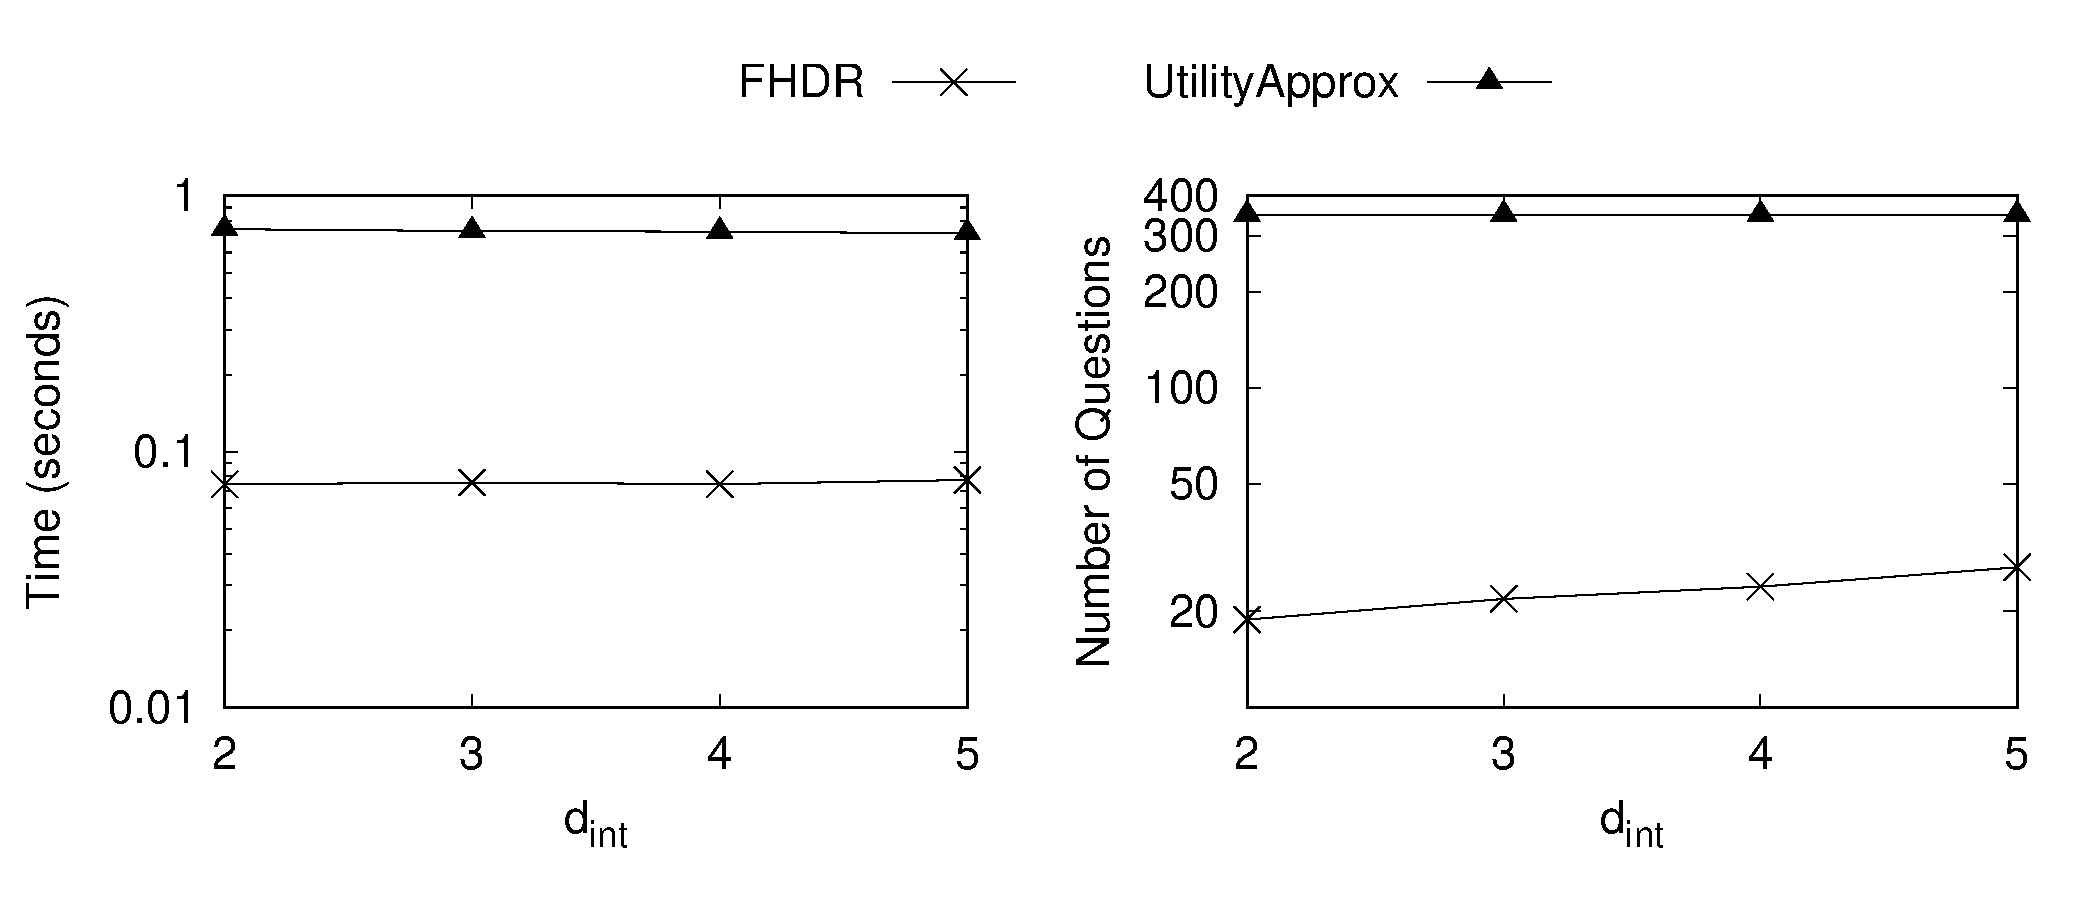
\includegraphics[width=0.67\linewidth]{plot/real/house/d_int_1_plots.pdf}
    \caption{P1: Vary $d_{\text{int}}$}
    \label{fig:house_a}
  \end{subfigure}
  \hfill
  \begin{subfigure}{0.48\linewidth}
    \centering
    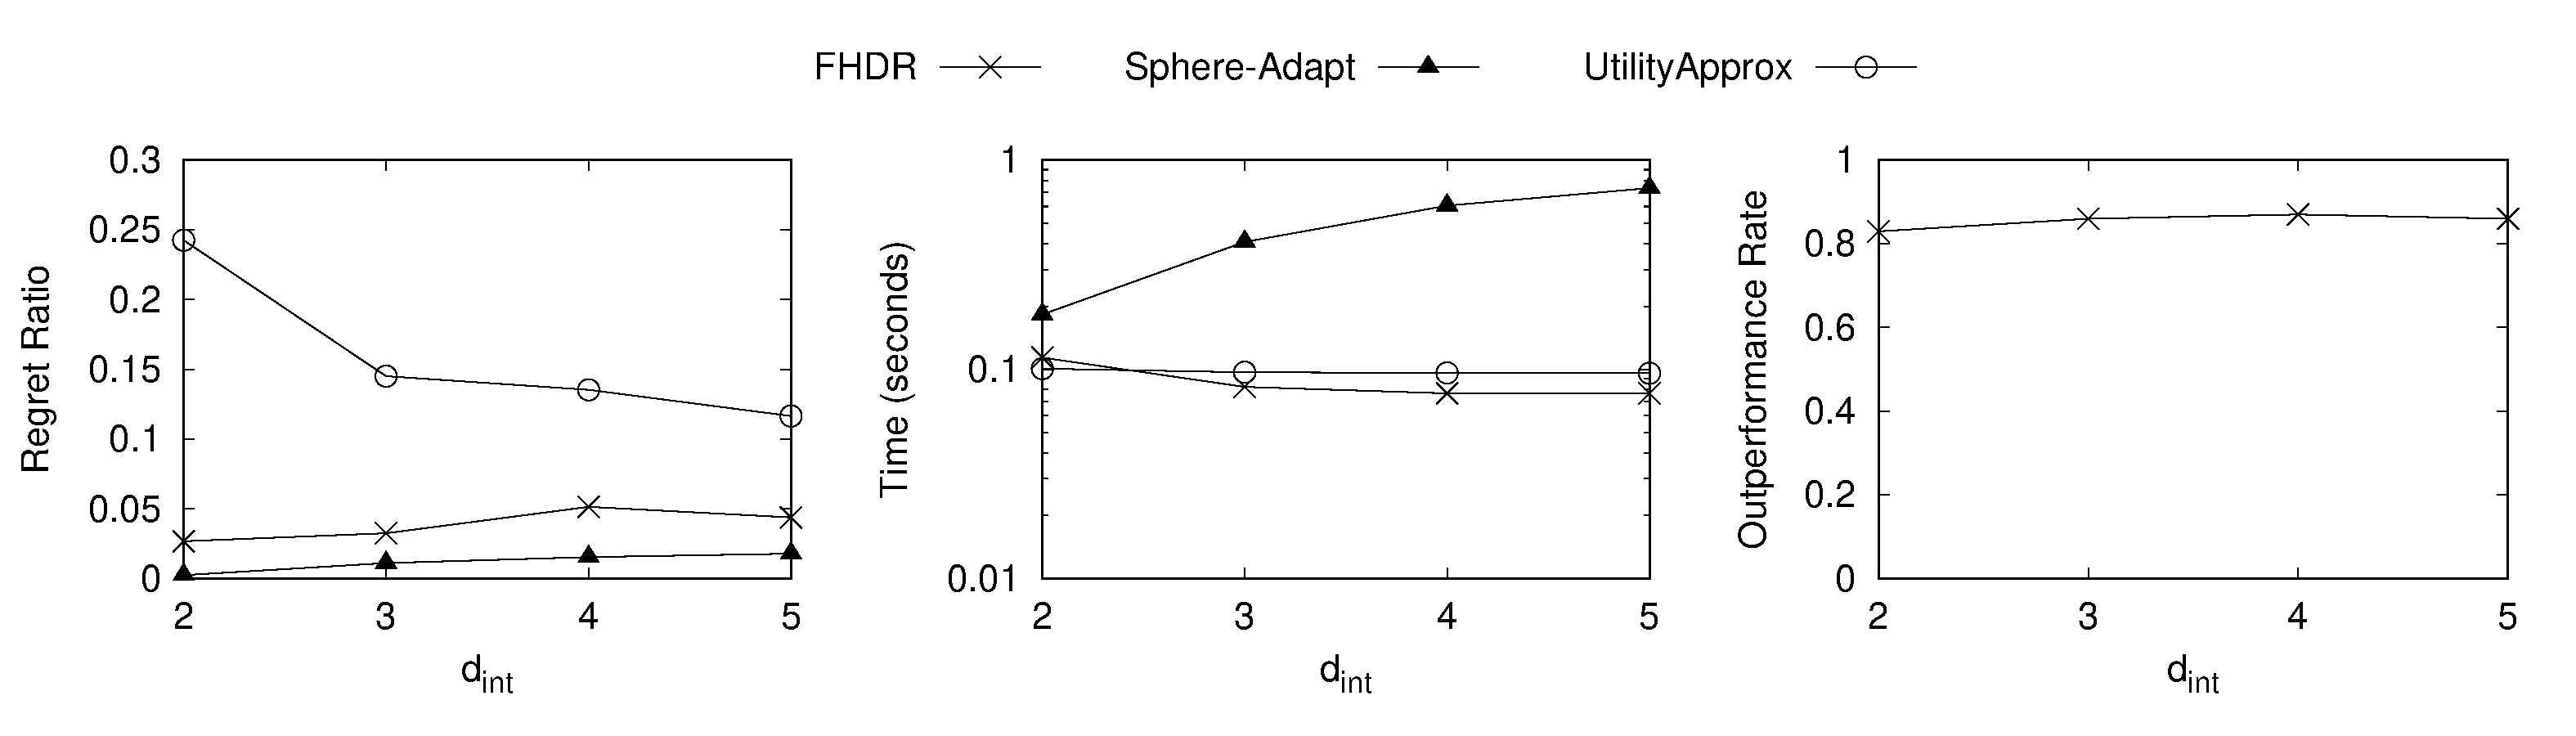
\includegraphics[width=\linewidth]{plot/real/house/d_int_2_plots.pdf}
    \caption{P2: Vary $d_{\text{int}}$}
    \label{fig:house_b}
  \end{subfigure}

  \vspace{0.6em}
  \begin{subfigure}{0.48\linewidth}
    \centering
    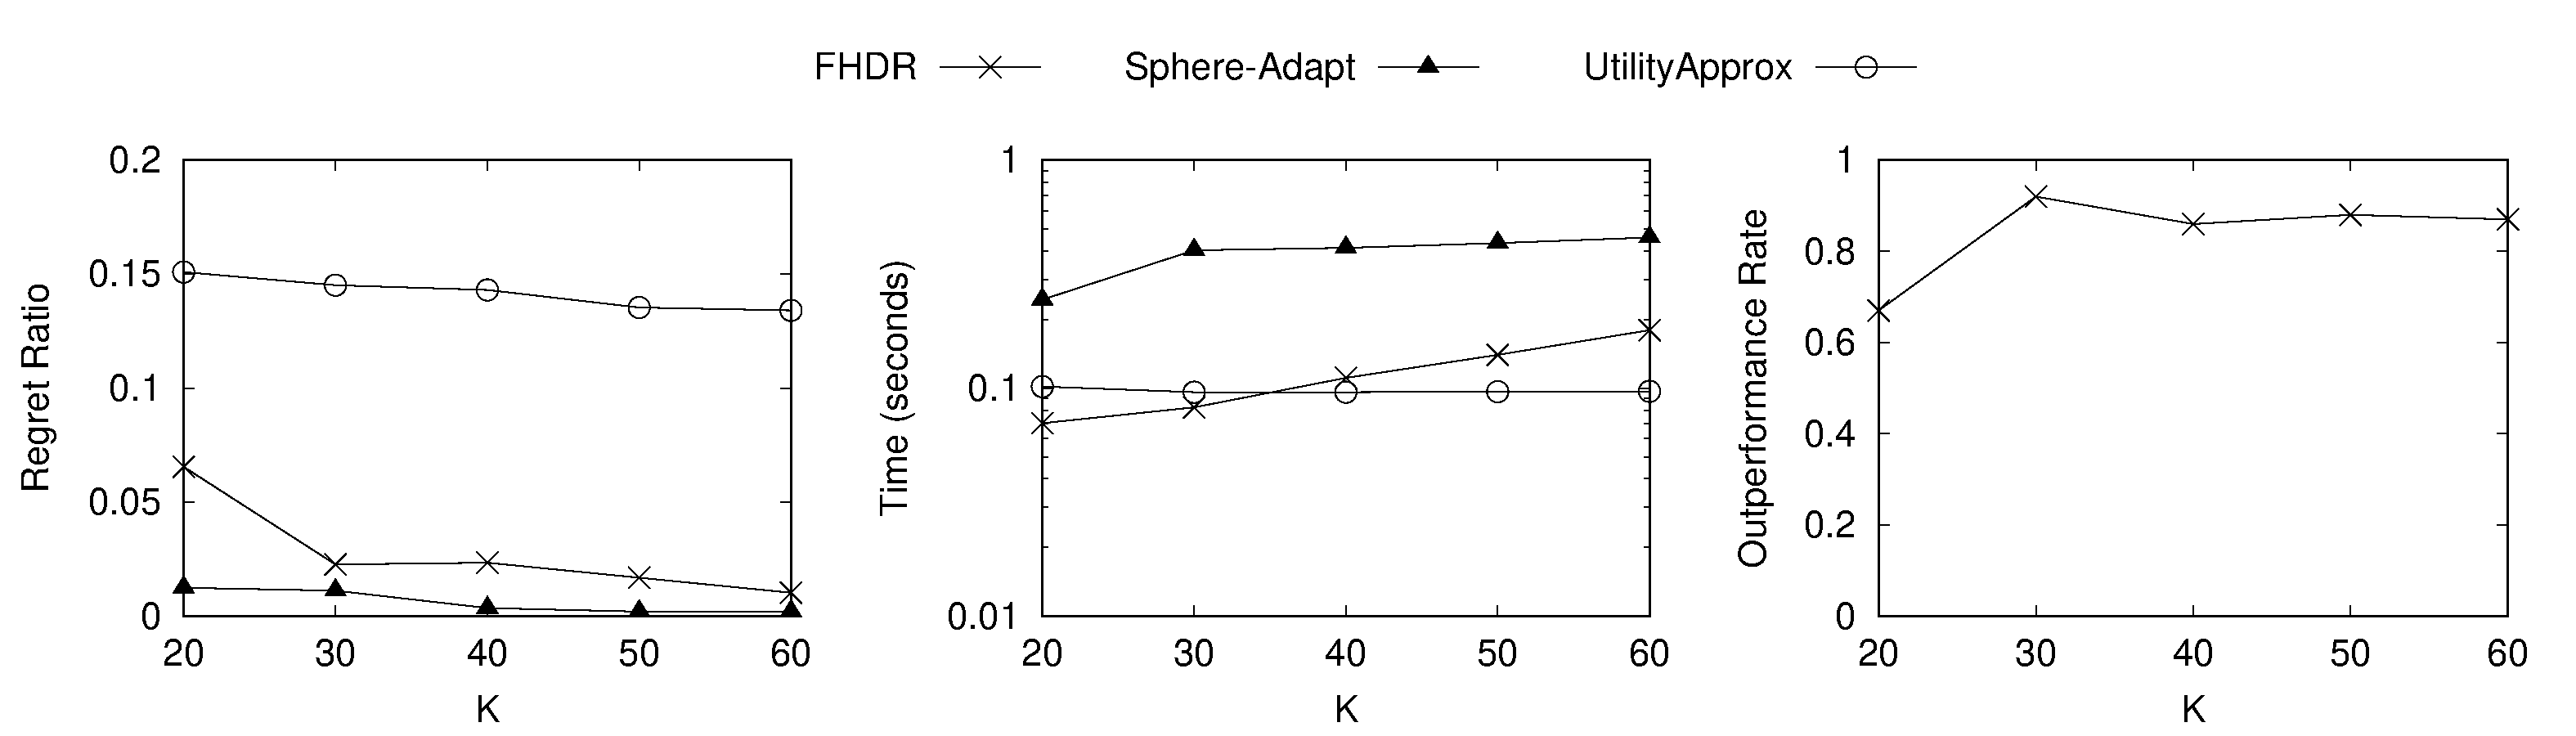
\includegraphics[width=\linewidth]{plot/real/house/K_plots.pdf}
    \caption{P2: Vary $K$}
    \label{fig:house_c}
  \end{subfigure}
  \hfill
  \begin{subfigure}{0.48\linewidth}
    \centering
    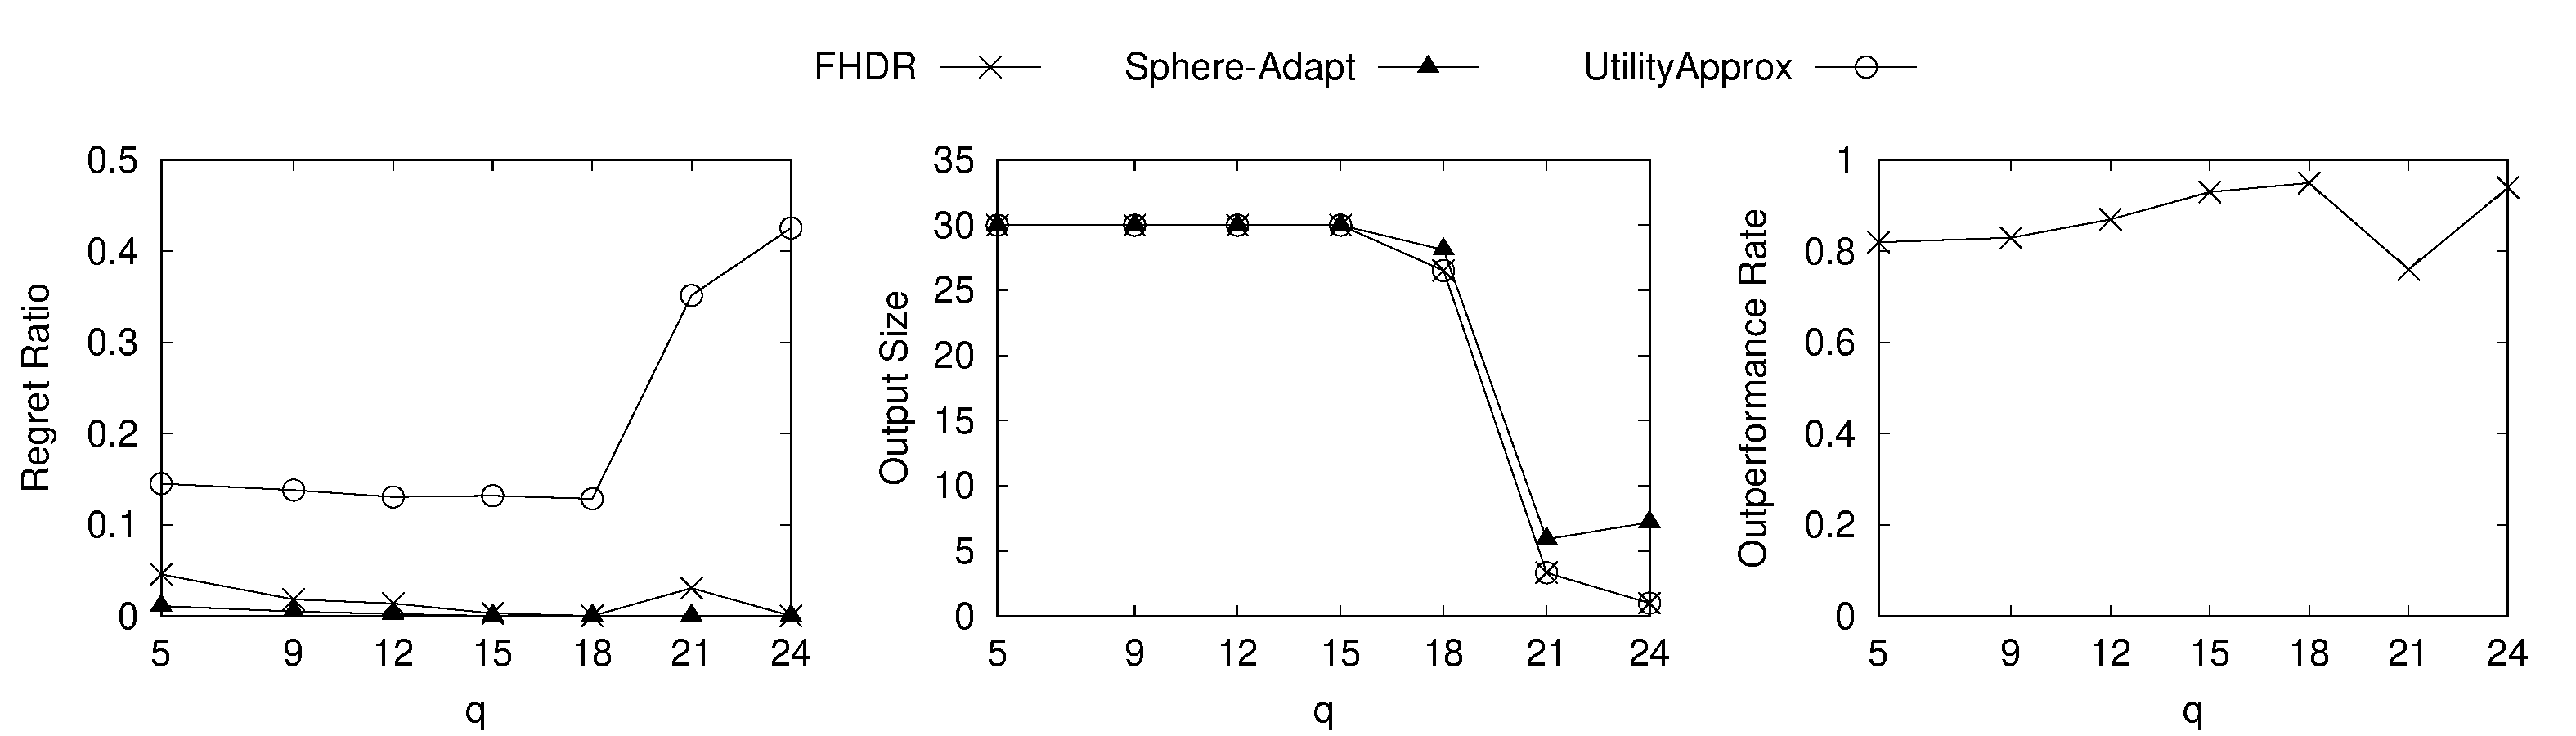
\includegraphics[width=\linewidth]{plot/real/house/q_plots.pdf}
    \caption{P2: Vary $q$}
    \label{fig:house_d}
  \end{subfigure}

  \caption{Results on \textit{House} dataset}
  \label{fig:house}
\end{figure*}

\begin{figure*}[tbp]
  \centering
  \begin{subfigure}{0.48\linewidth}
    \centering
    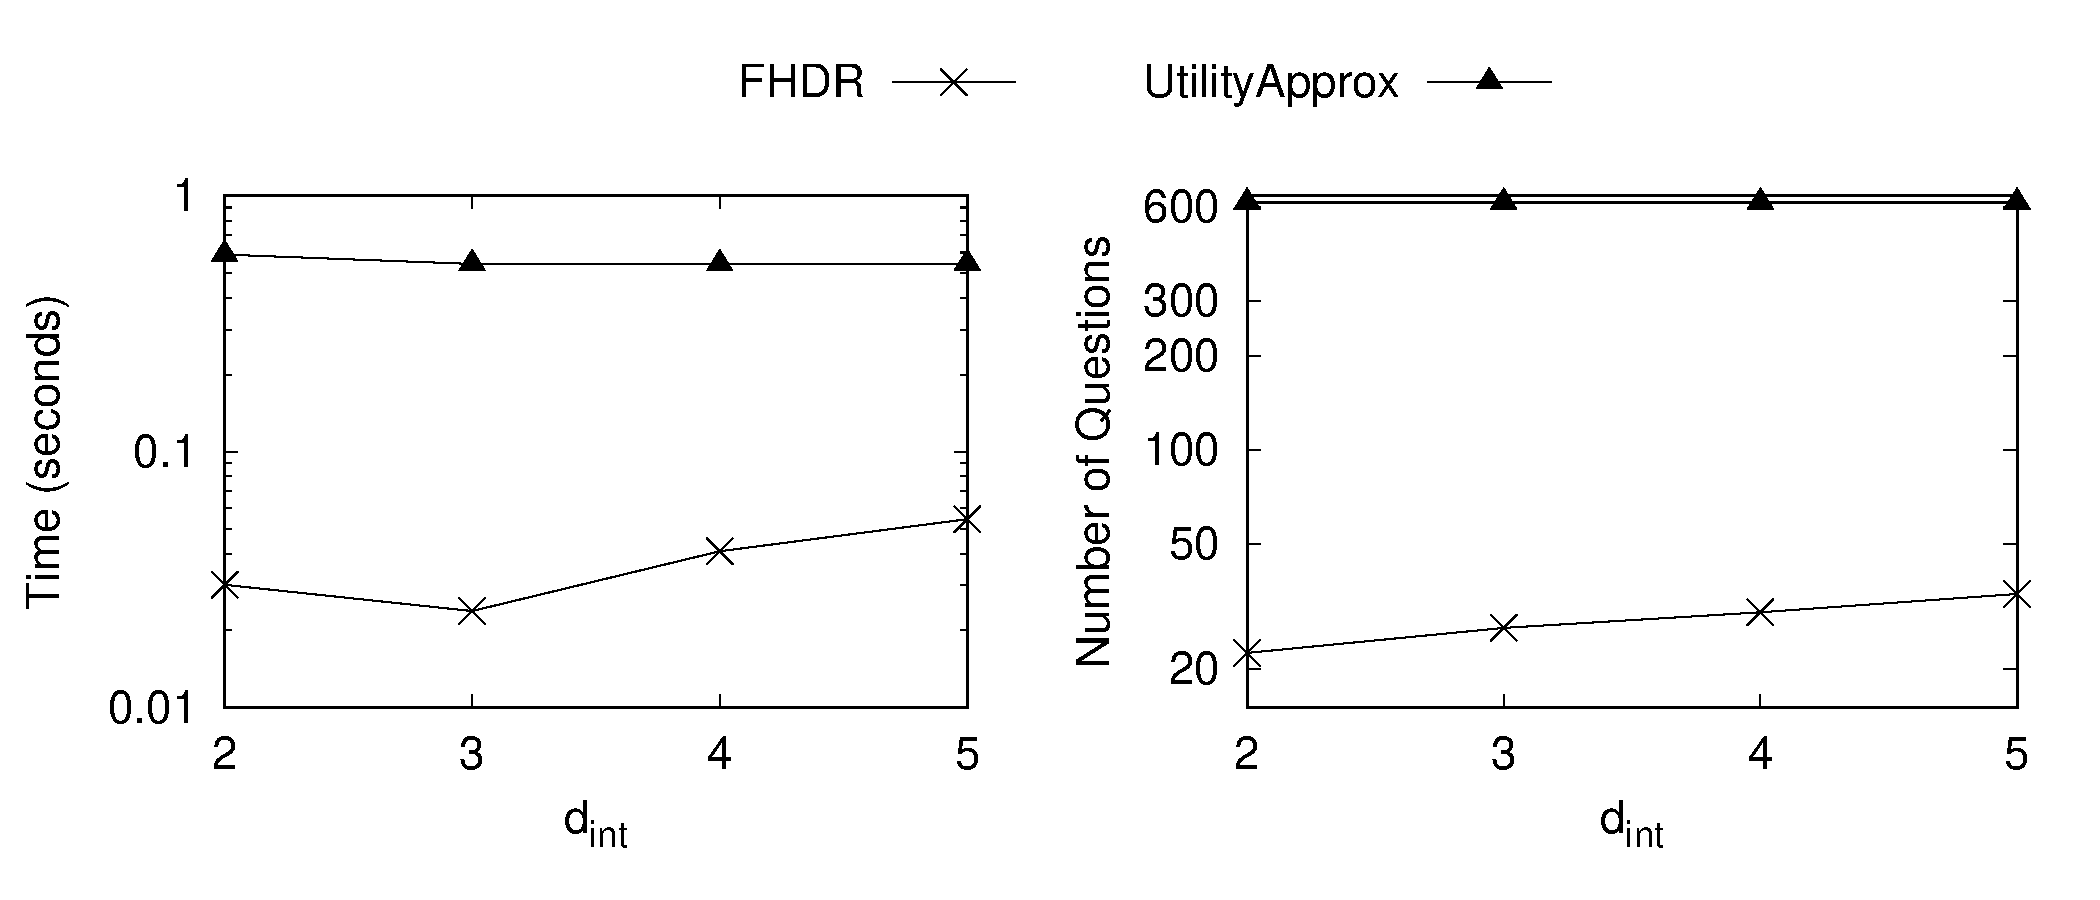
\includegraphics[width=0.67\linewidth]{plot/real/car/d_int_1_plots.pdf}
    \caption{P1: Vary $d_{\text{int}}$}
    \label{fig:car_a}
  \end{subfigure}
  \hfill
  \begin{subfigure}{0.48\linewidth}
    \centering
    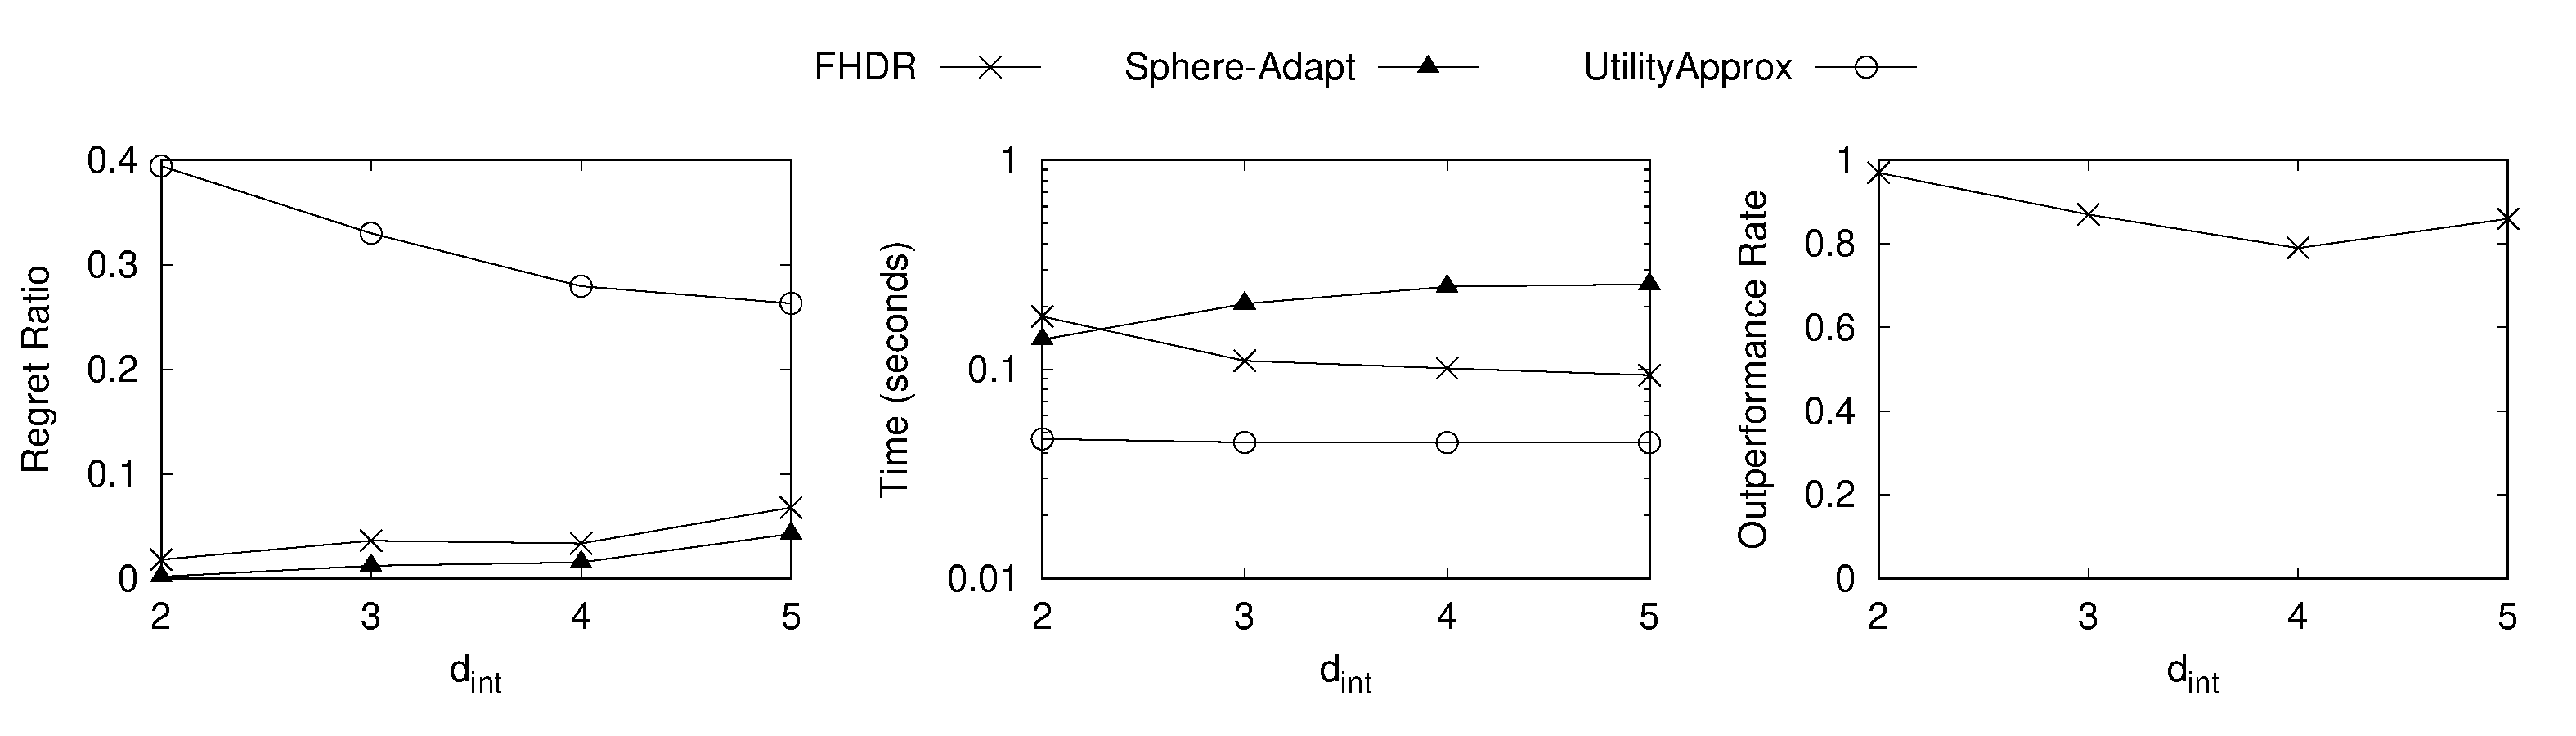
\includegraphics[width=\linewidth]{plot/real/car/d_int_2_plots.pdf}
    \caption{P2: Vary $d_{\text{int}}$}
    \label{fig:car_b}
  \end{subfigure}

  \vspace{0.6em}
  \begin{subfigure}{0.48\linewidth}
    \centering
    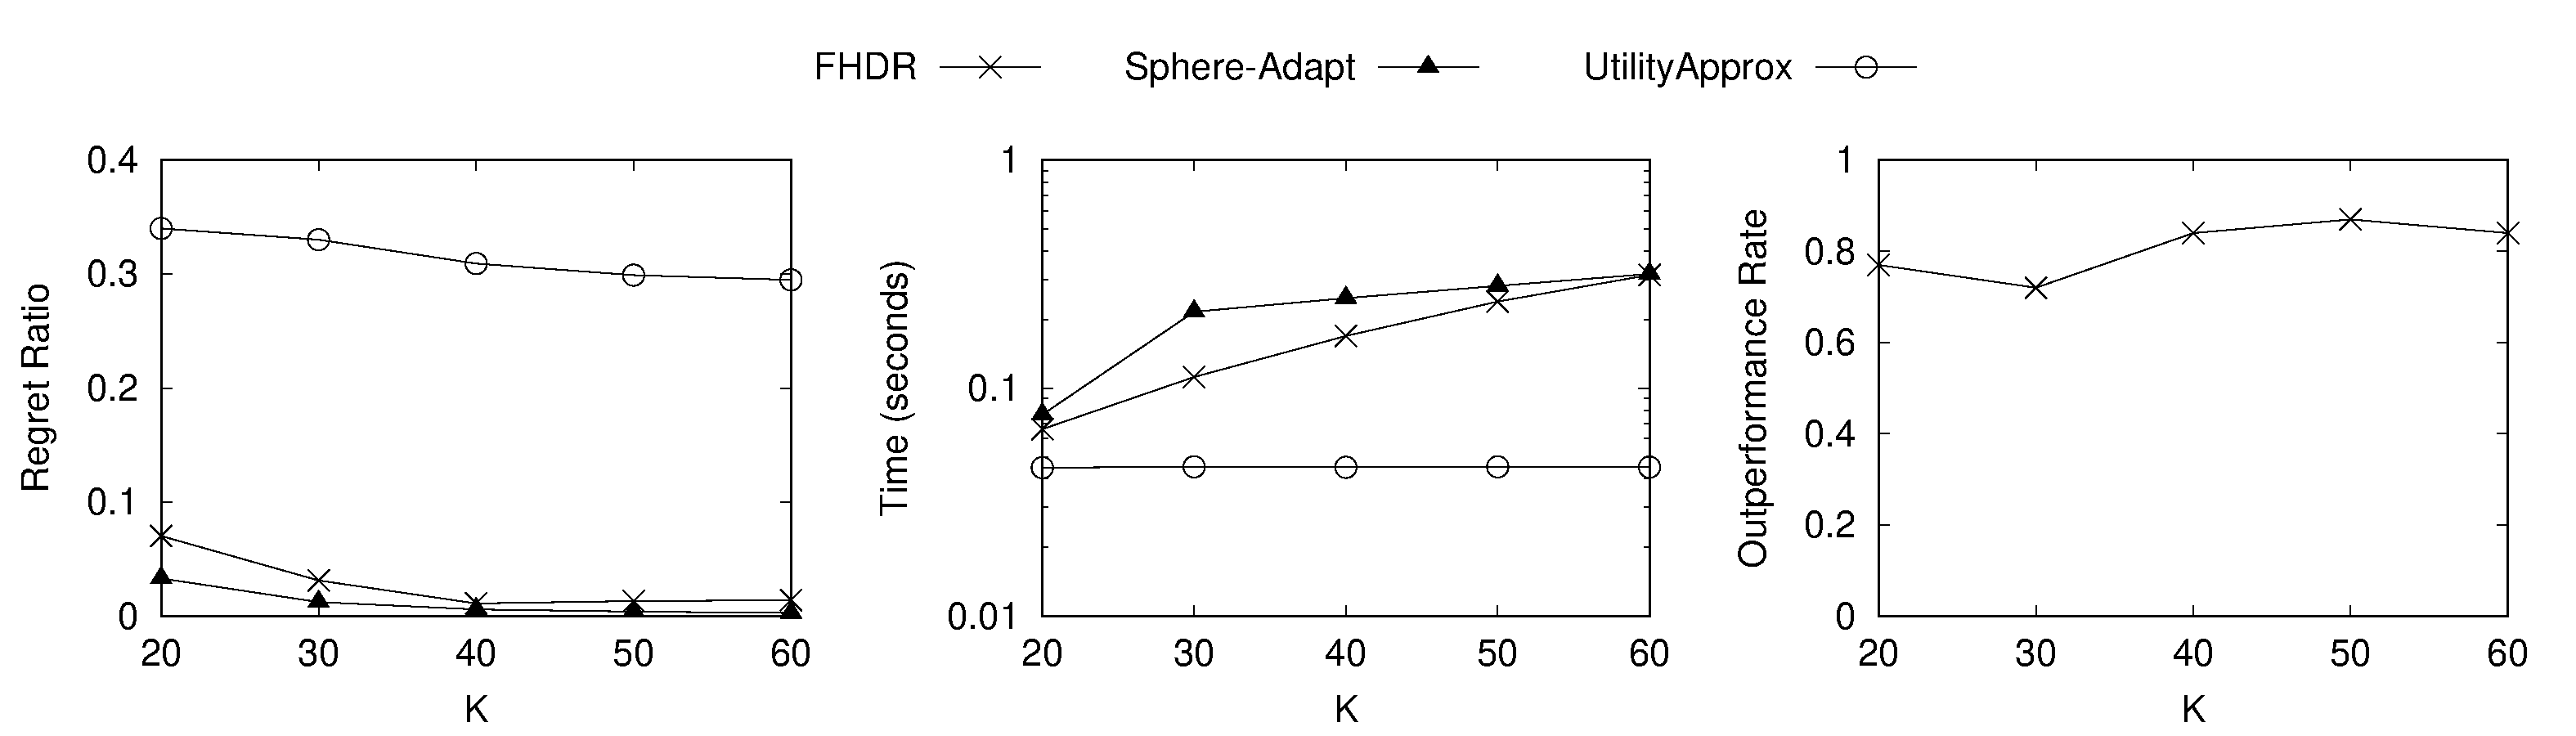
\includegraphics[width=\linewidth]{plot/real/car/K_plots.pdf}
    \caption{P2: Vary $K$}
    \label{fig:car_c}
  \end{subfigure}
  \hfill
  \begin{subfigure}{0.48\linewidth}
    \centering
    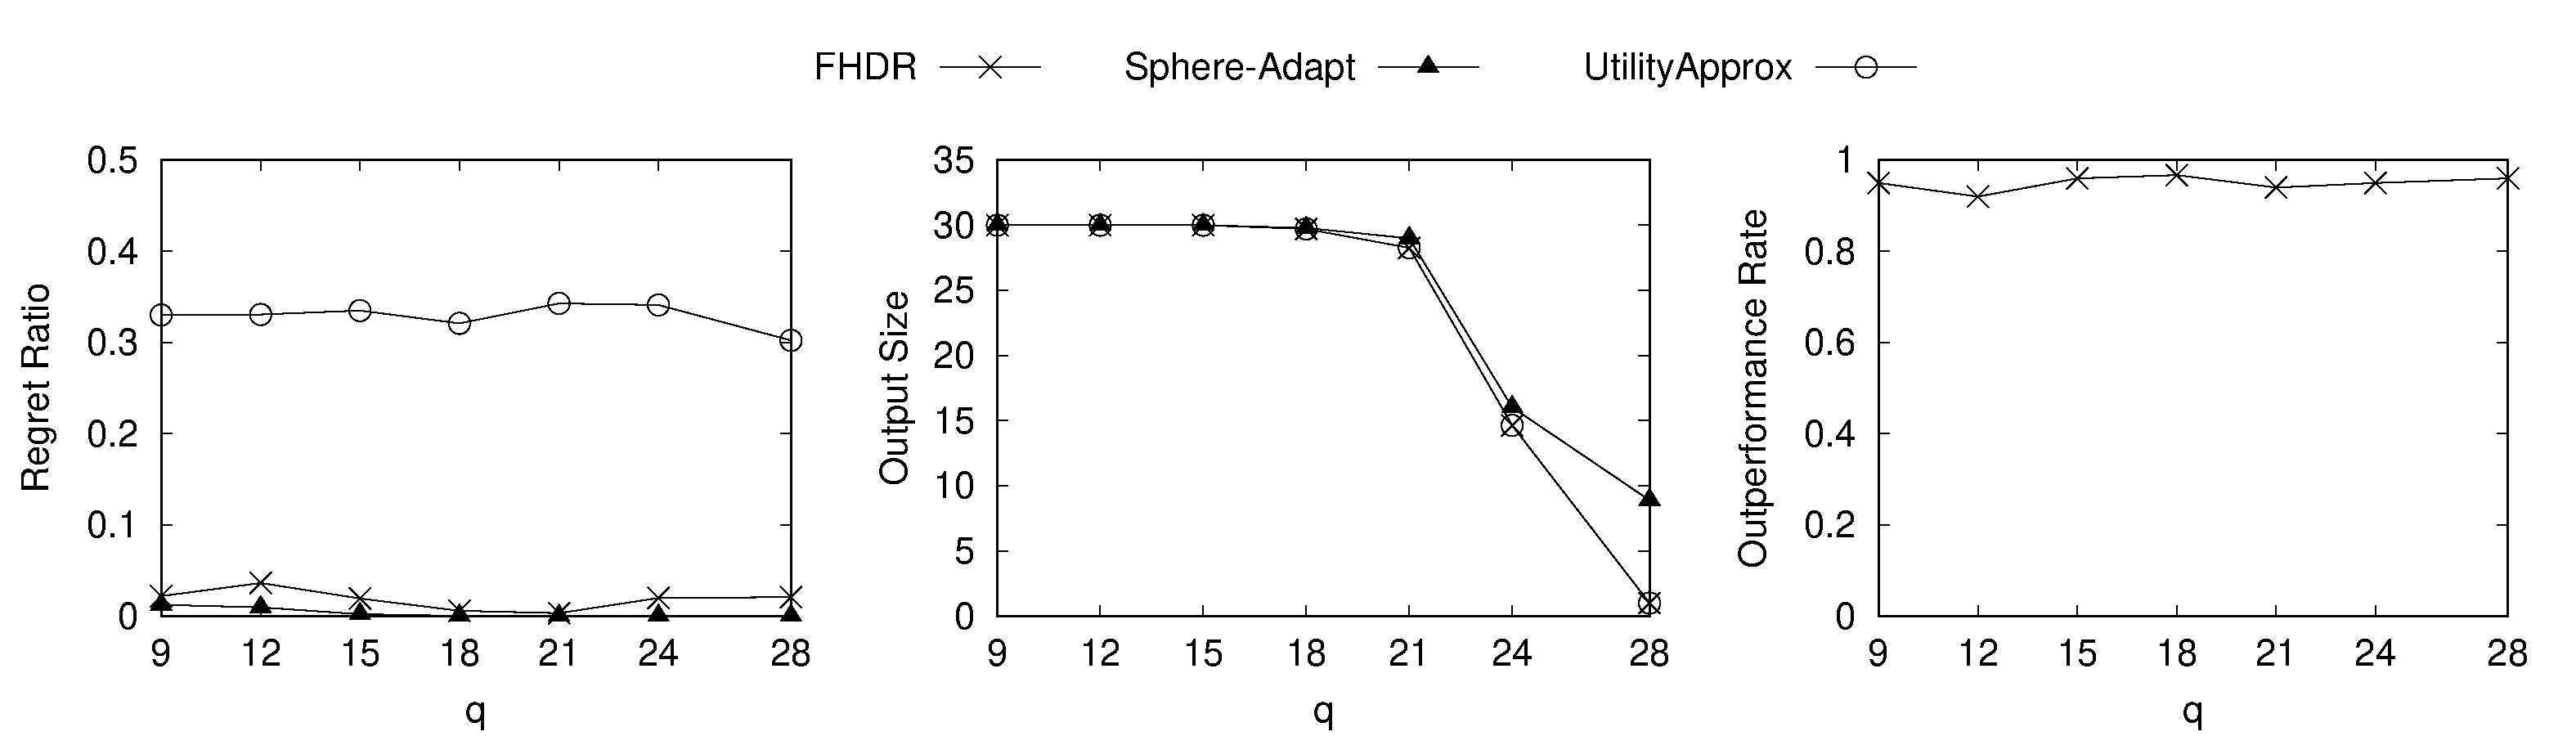
\includegraphics[width=\linewidth]{plot/real/car/q_plots.pdf}
    \caption{P2: Vary $q$}
    \label{fig:car_d}
  \end{subfigure}

  \caption{Results on \textit{Car} dataset}
  \label{fig:car}
\end{figure*}

\begin{figure*}[tbp]
  \centering
  \begin{subfigure}{0.48\linewidth}
    \centering
    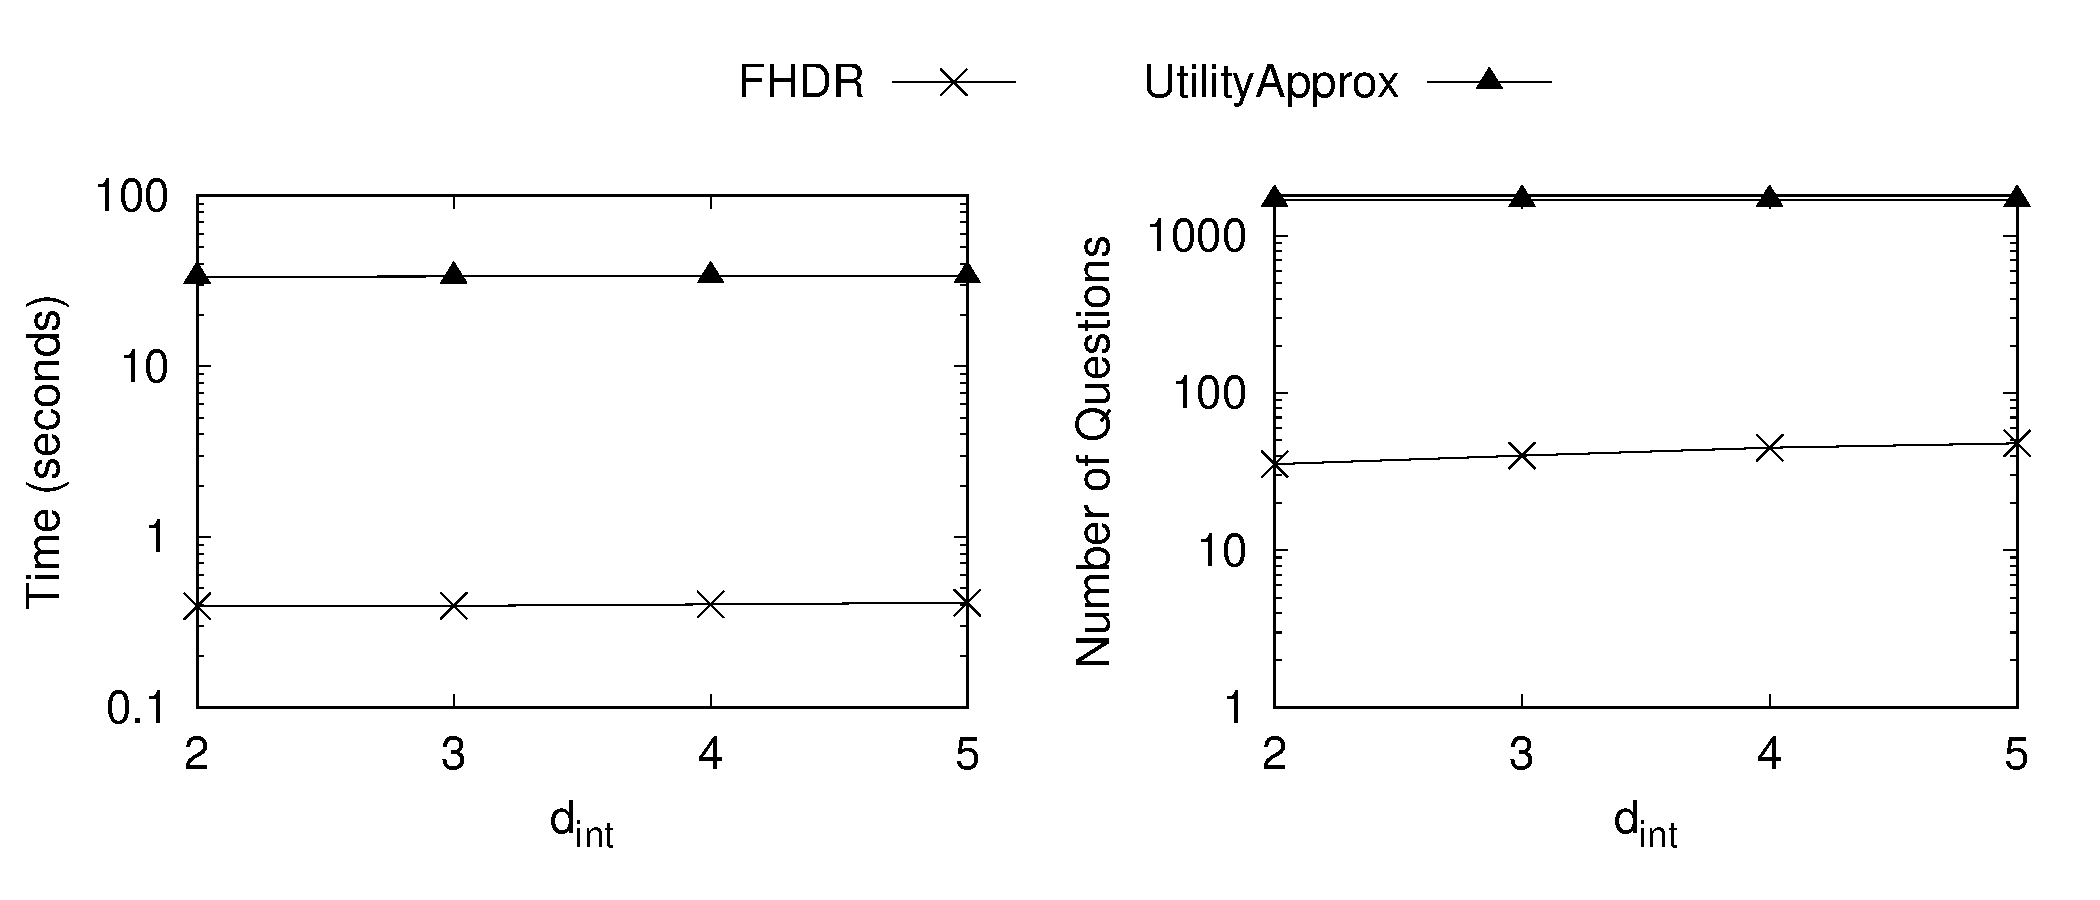
\includegraphics[width=0.67\linewidth]{plot/real/energy/d_int_1_plots.pdf}
    \caption{P1: Vary $d_{\text{int}}$}
    \label{fig:energy_a}
  \end{subfigure}
  \hfill
  \begin{subfigure}{0.48\linewidth}
    \centering
    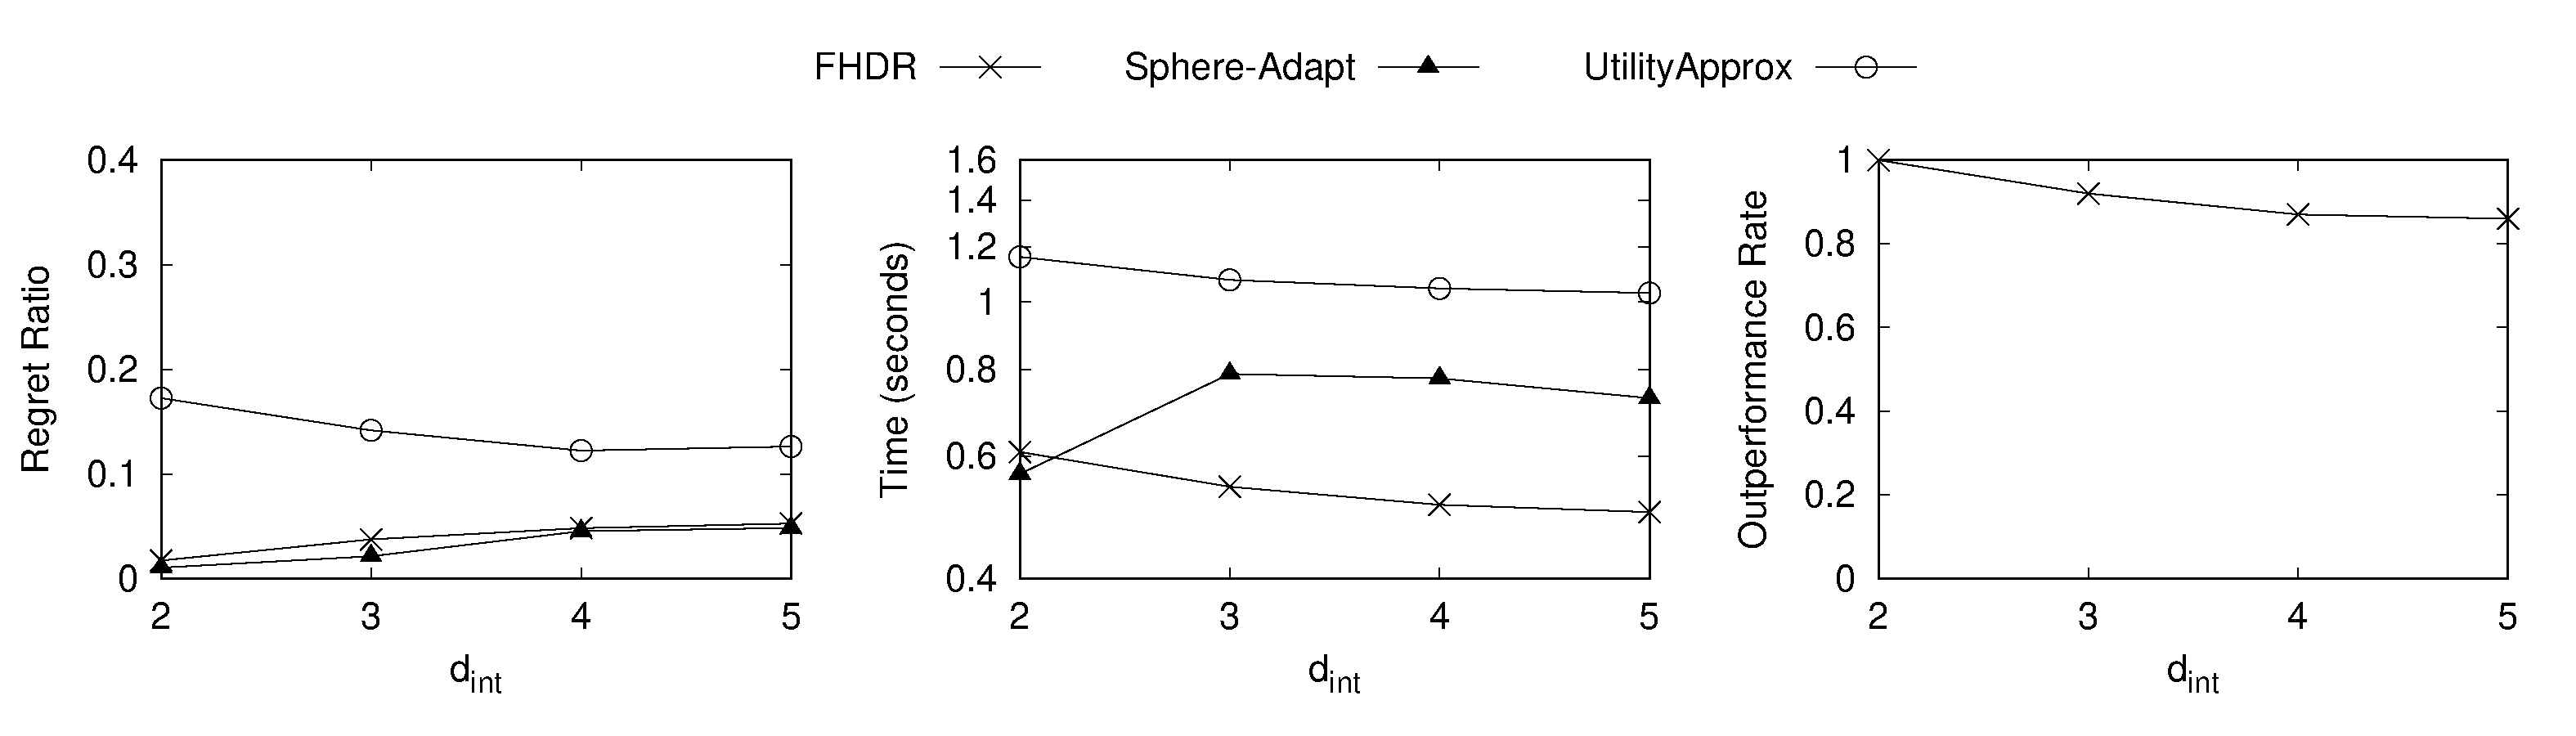
\includegraphics[width=\linewidth]{plot/real/energy/d_int_2_plots.pdf}
    \caption{P2: Vary $d_{\text{int}}$}
    \label{fig:energy_b}
  \end{subfigure}

  \vspace{0.6em}
  \begin{subfigure}{0.48\linewidth}
    \centering
    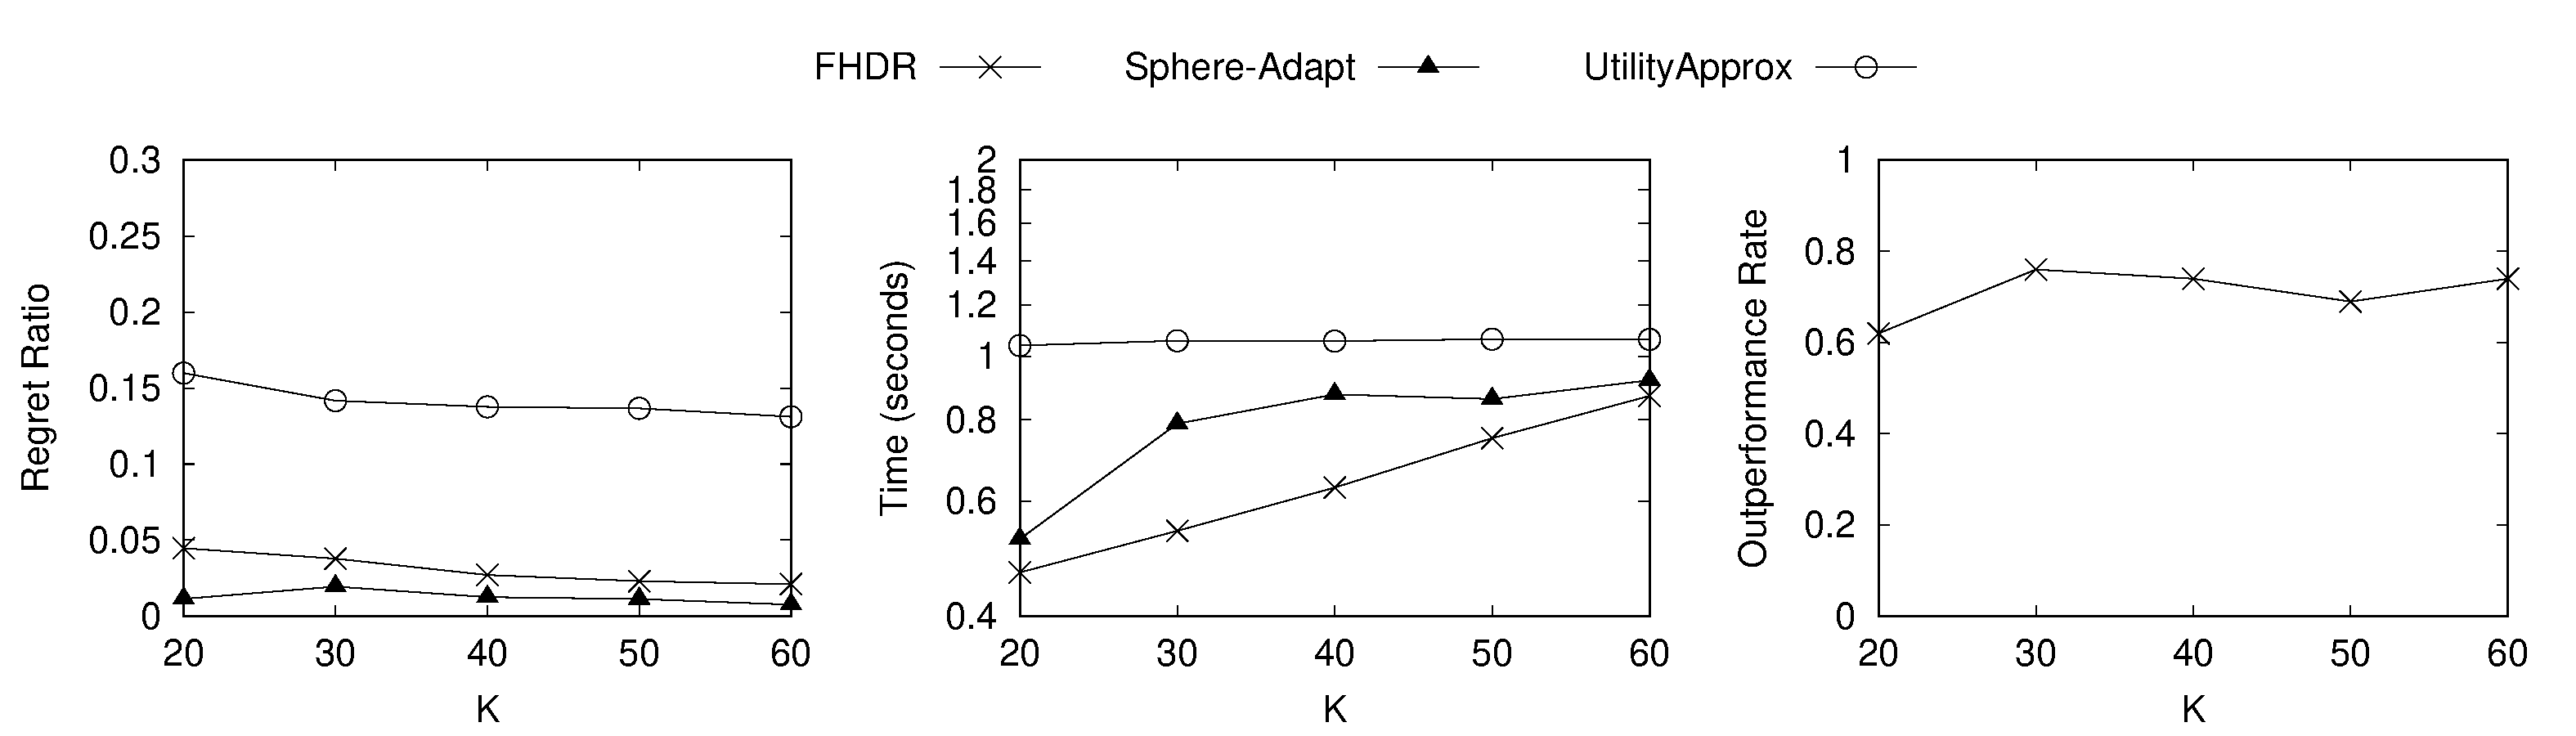
\includegraphics[width=\linewidth]{plot/real/energy/K_plots.pdf}
    \caption{P2: Vary $K$}
    \label{fig:energy_c}
  \end{subfigure}
  \hfill
  \begin{subfigure}{0.48\linewidth}
    \centering
    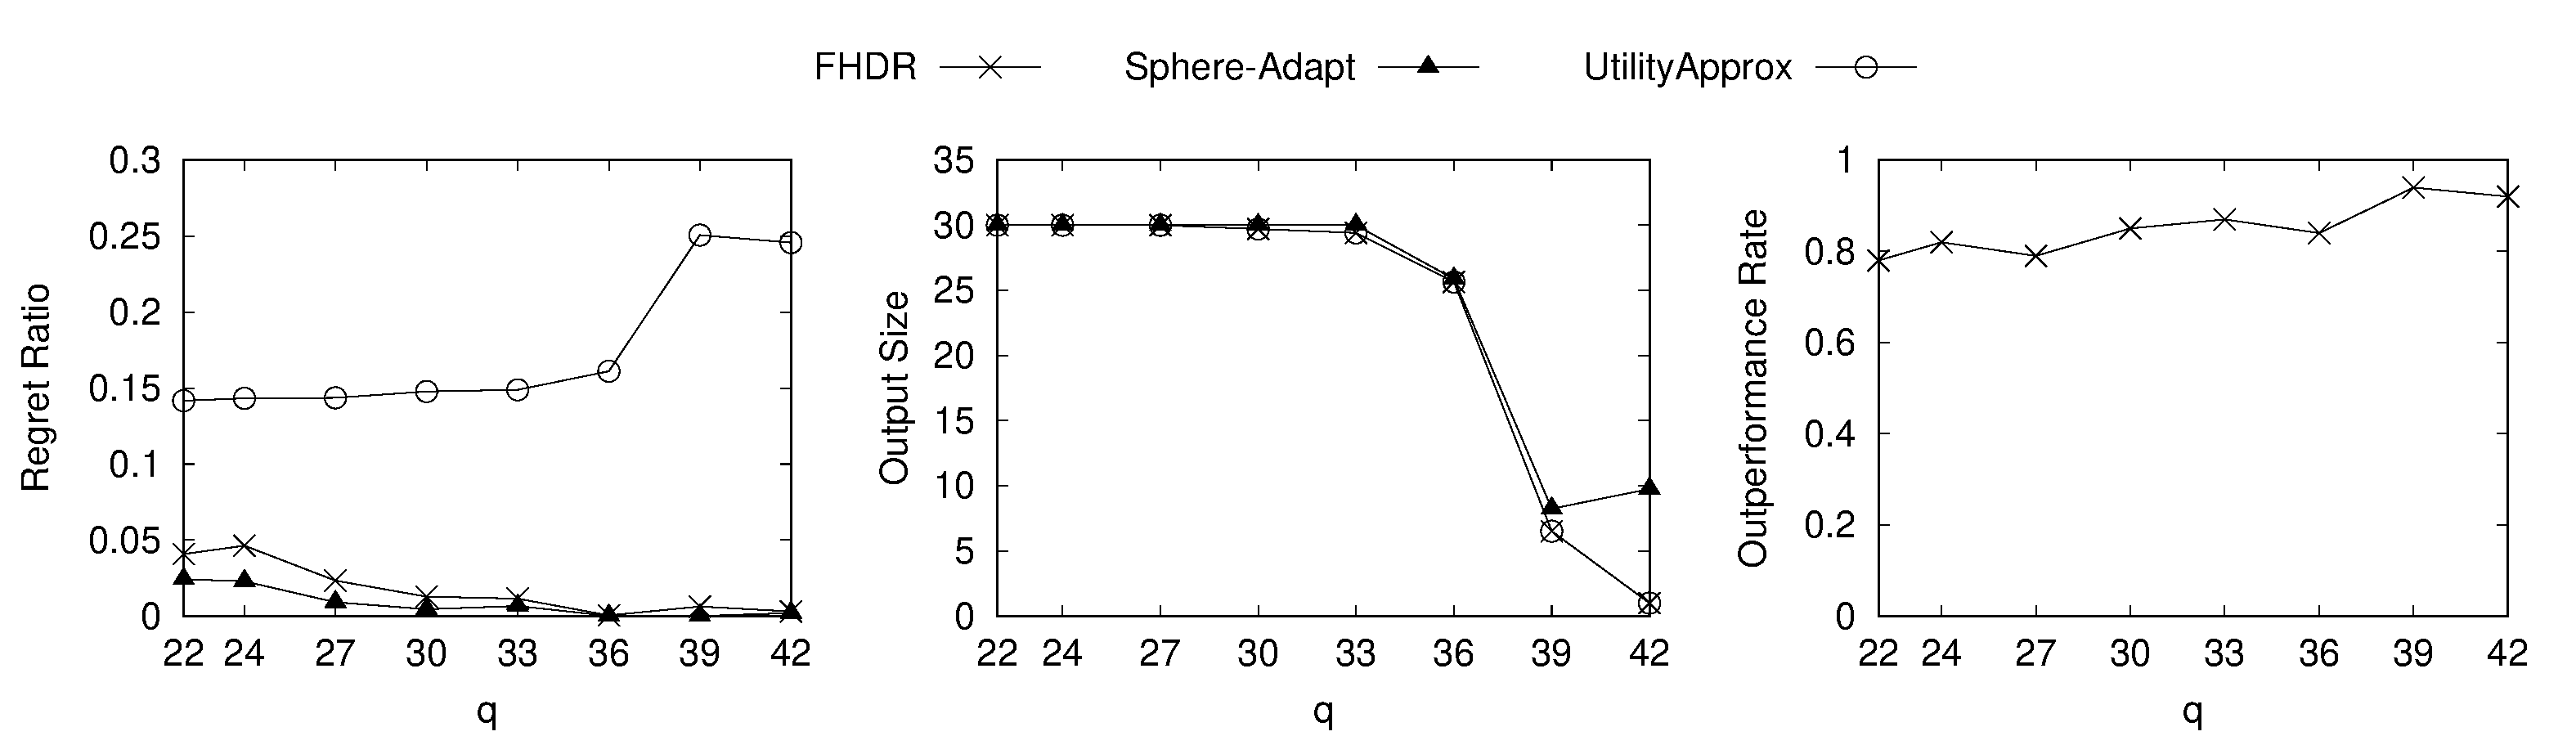
\includegraphics[width=\linewidth]{plot/real/energy/q_plots.pdf}
    \caption{P2: Vary $q$}
    \label{fig:energy_d}
  \end{subfigure}

  \caption{Results on \textit{Energy} dataset}
  \label{fig:energy}
\end{figure*}

\begin{figure*}[tbp]
  \centering
  \begin{subfigure}{0.48\linewidth}
    \centering
    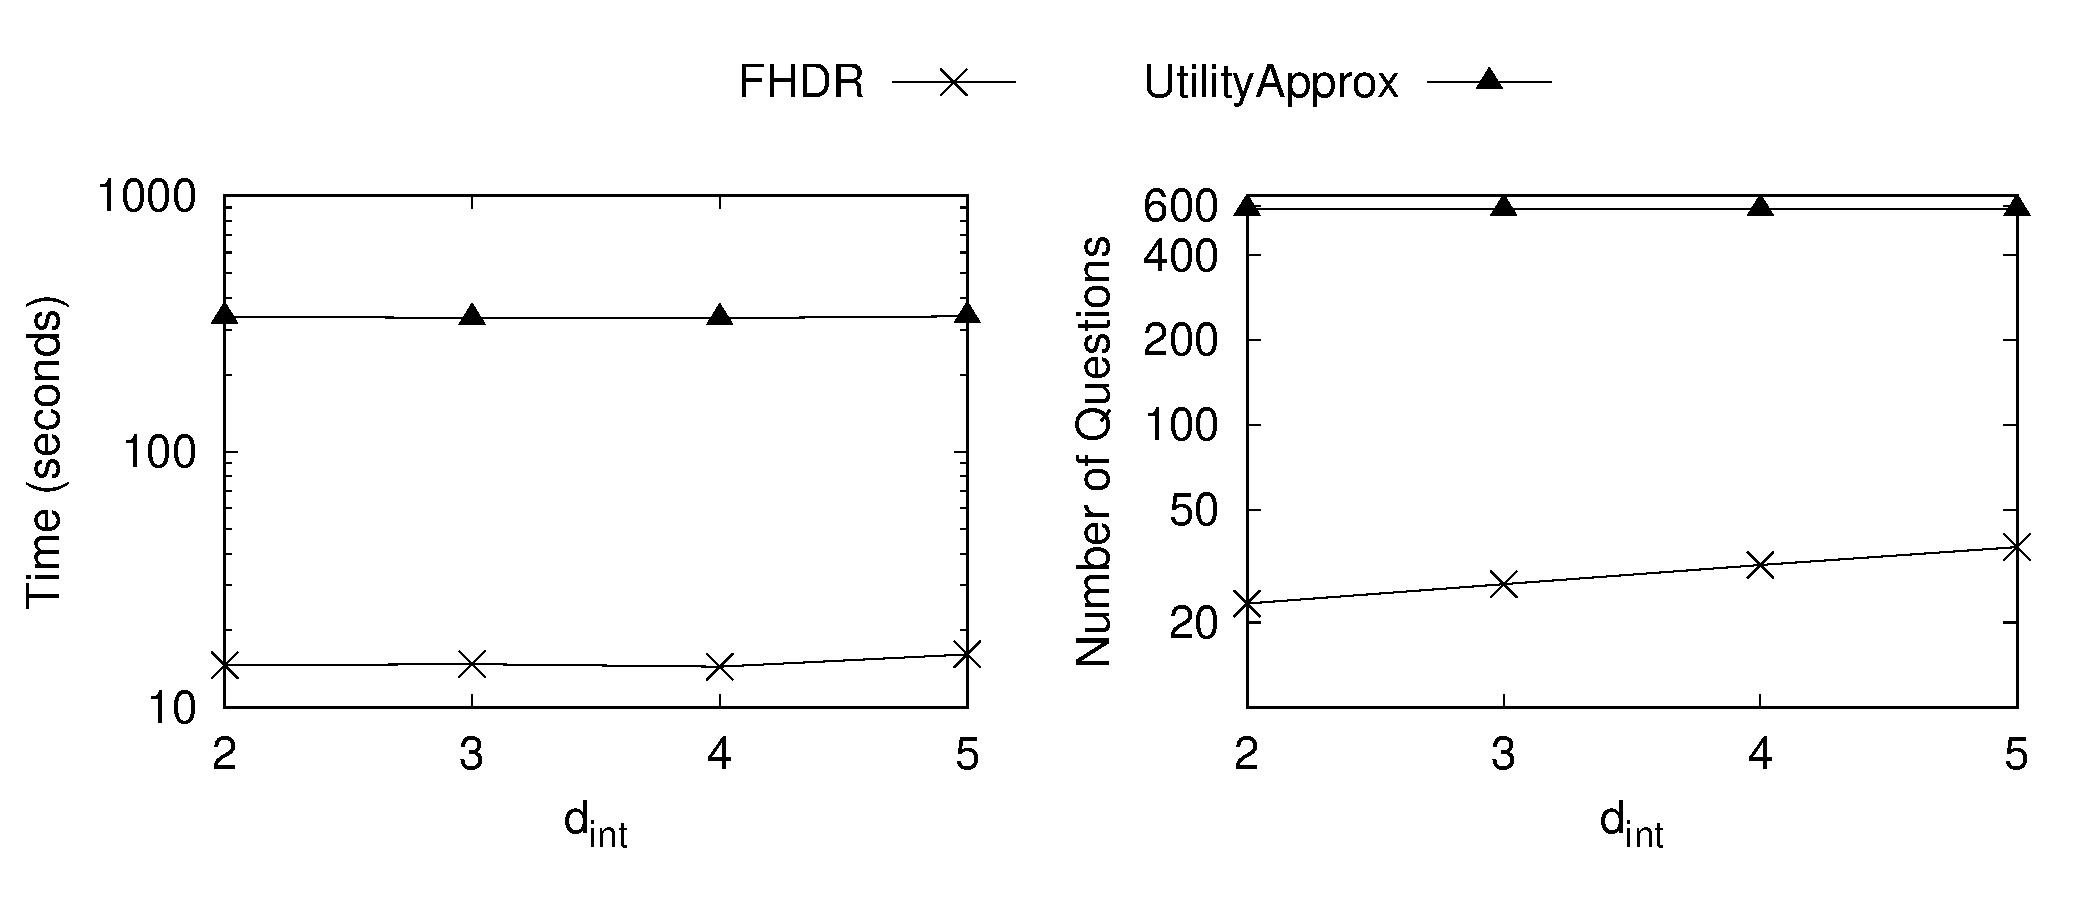
\includegraphics[width=0.67\linewidth]{plot/real/activity/d_int_1_plots.pdf}
    \caption{P1: Vary $d_{\text{int}}$}
    \label{fig:activity_a}
  \end{subfigure}
  \hfill
  \begin{subfigure}{0.48\linewidth}
    \centering
    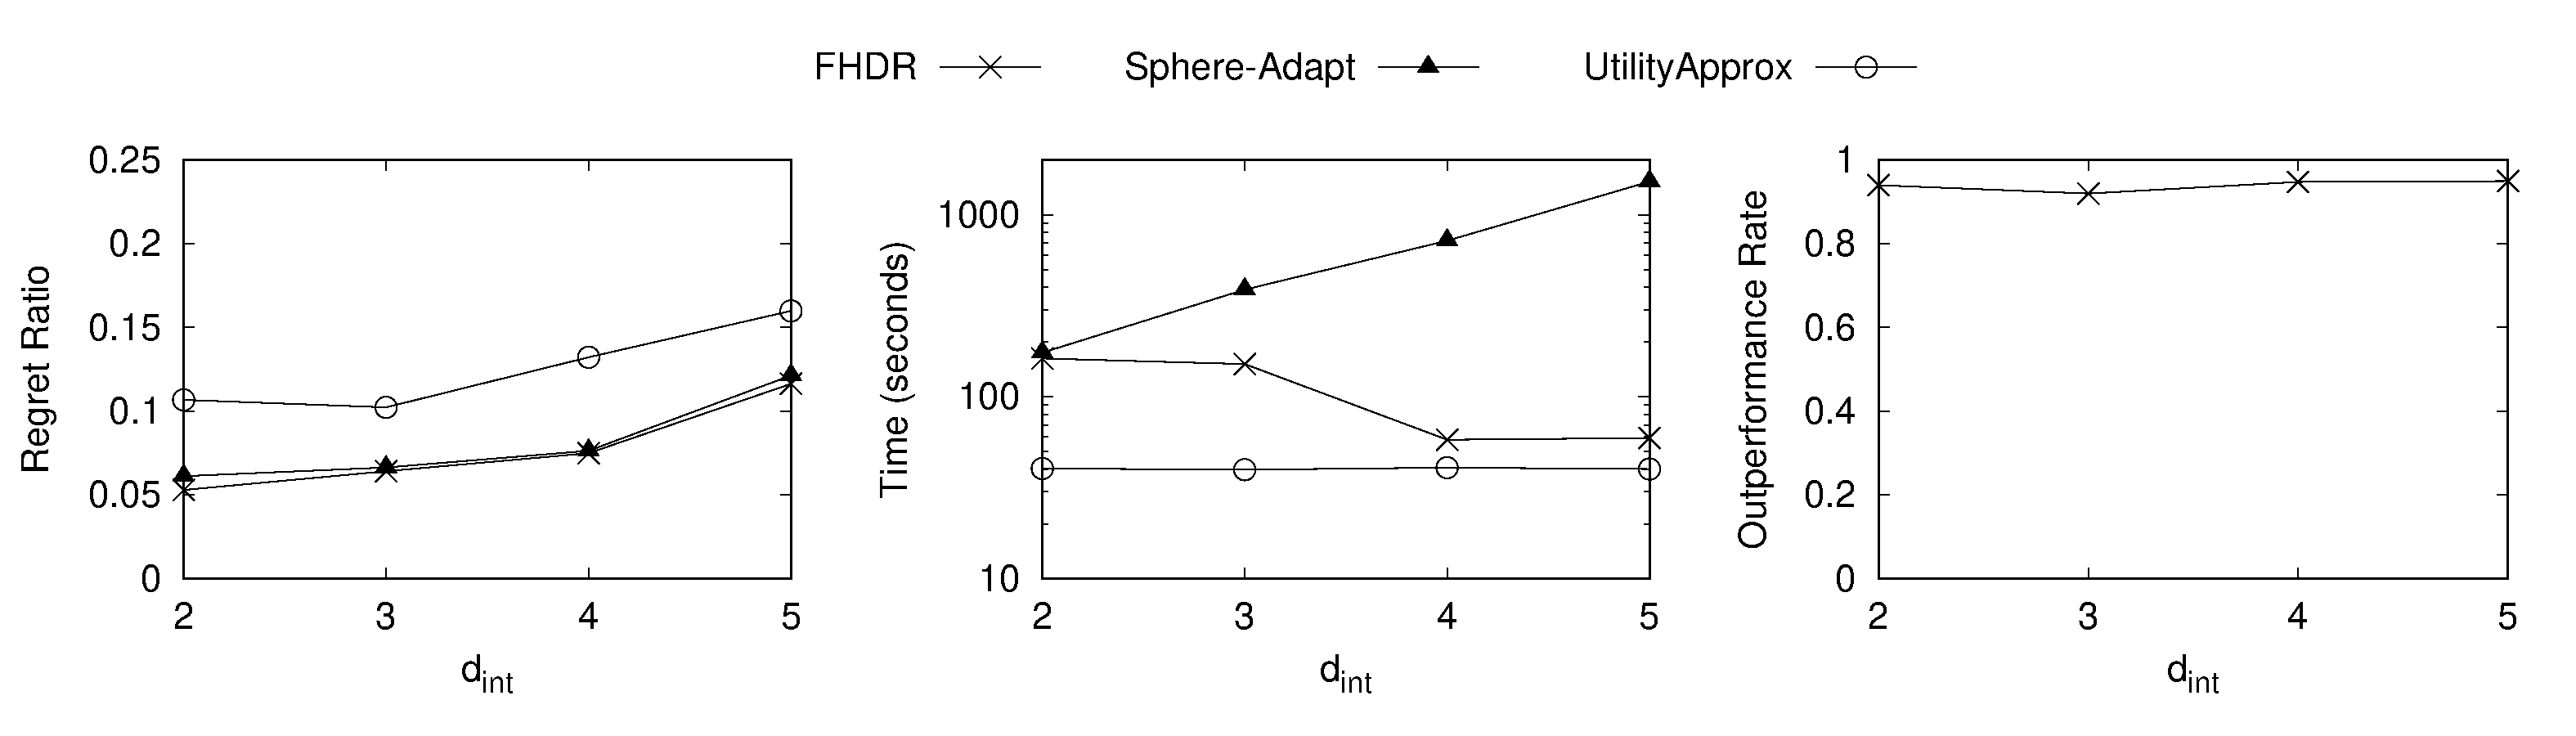
\includegraphics[width=\linewidth]{plot/real/activity/d_int_2_plots.pdf}
    \caption{P2: Vary $d_{\text{int}}$}
    \label{fig:activity_b}
  \end{subfigure}

  \vspace{0.6em}
  \begin{subfigure}{0.48\linewidth}
    \centering
    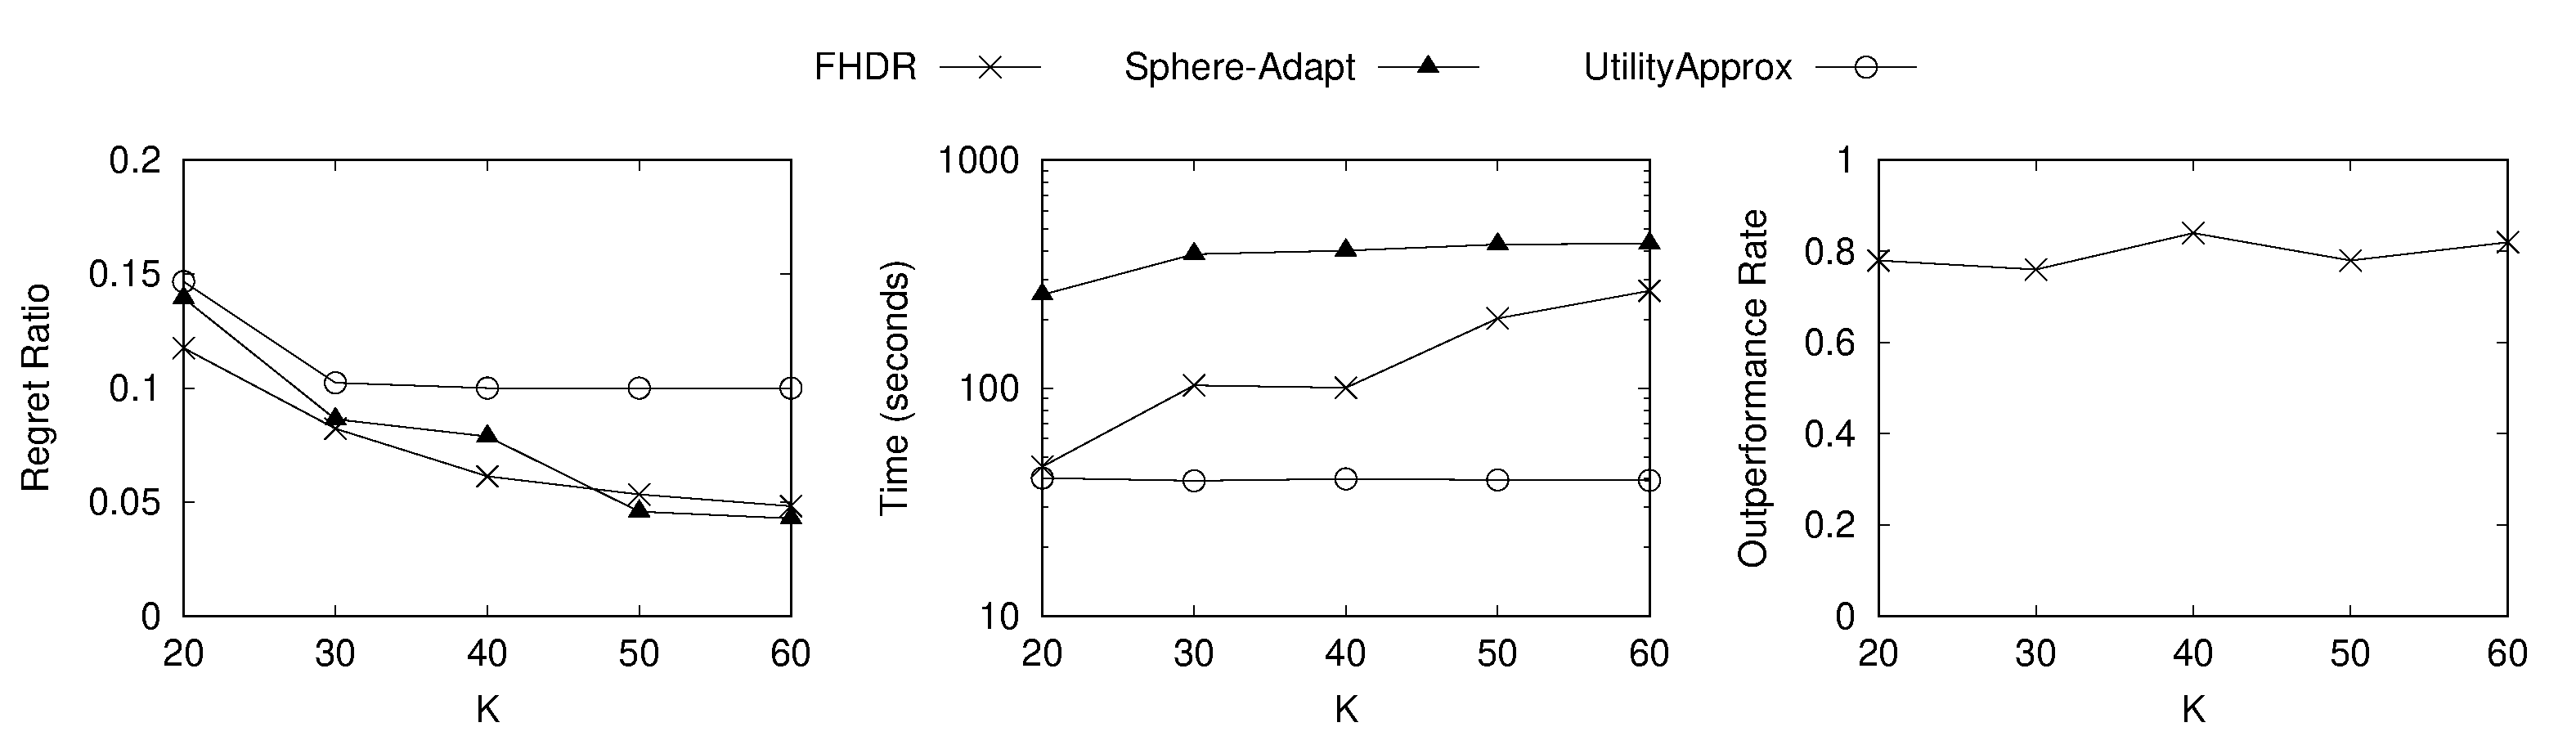
\includegraphics[width=\linewidth]{plot/real/activity/K_plots.pdf}
    \caption{P2: Vary $K$}
    \label{fig:activity_c}
  \end{subfigure}
  \hfill
  \begin{subfigure}{0.48\linewidth}
    \centering
    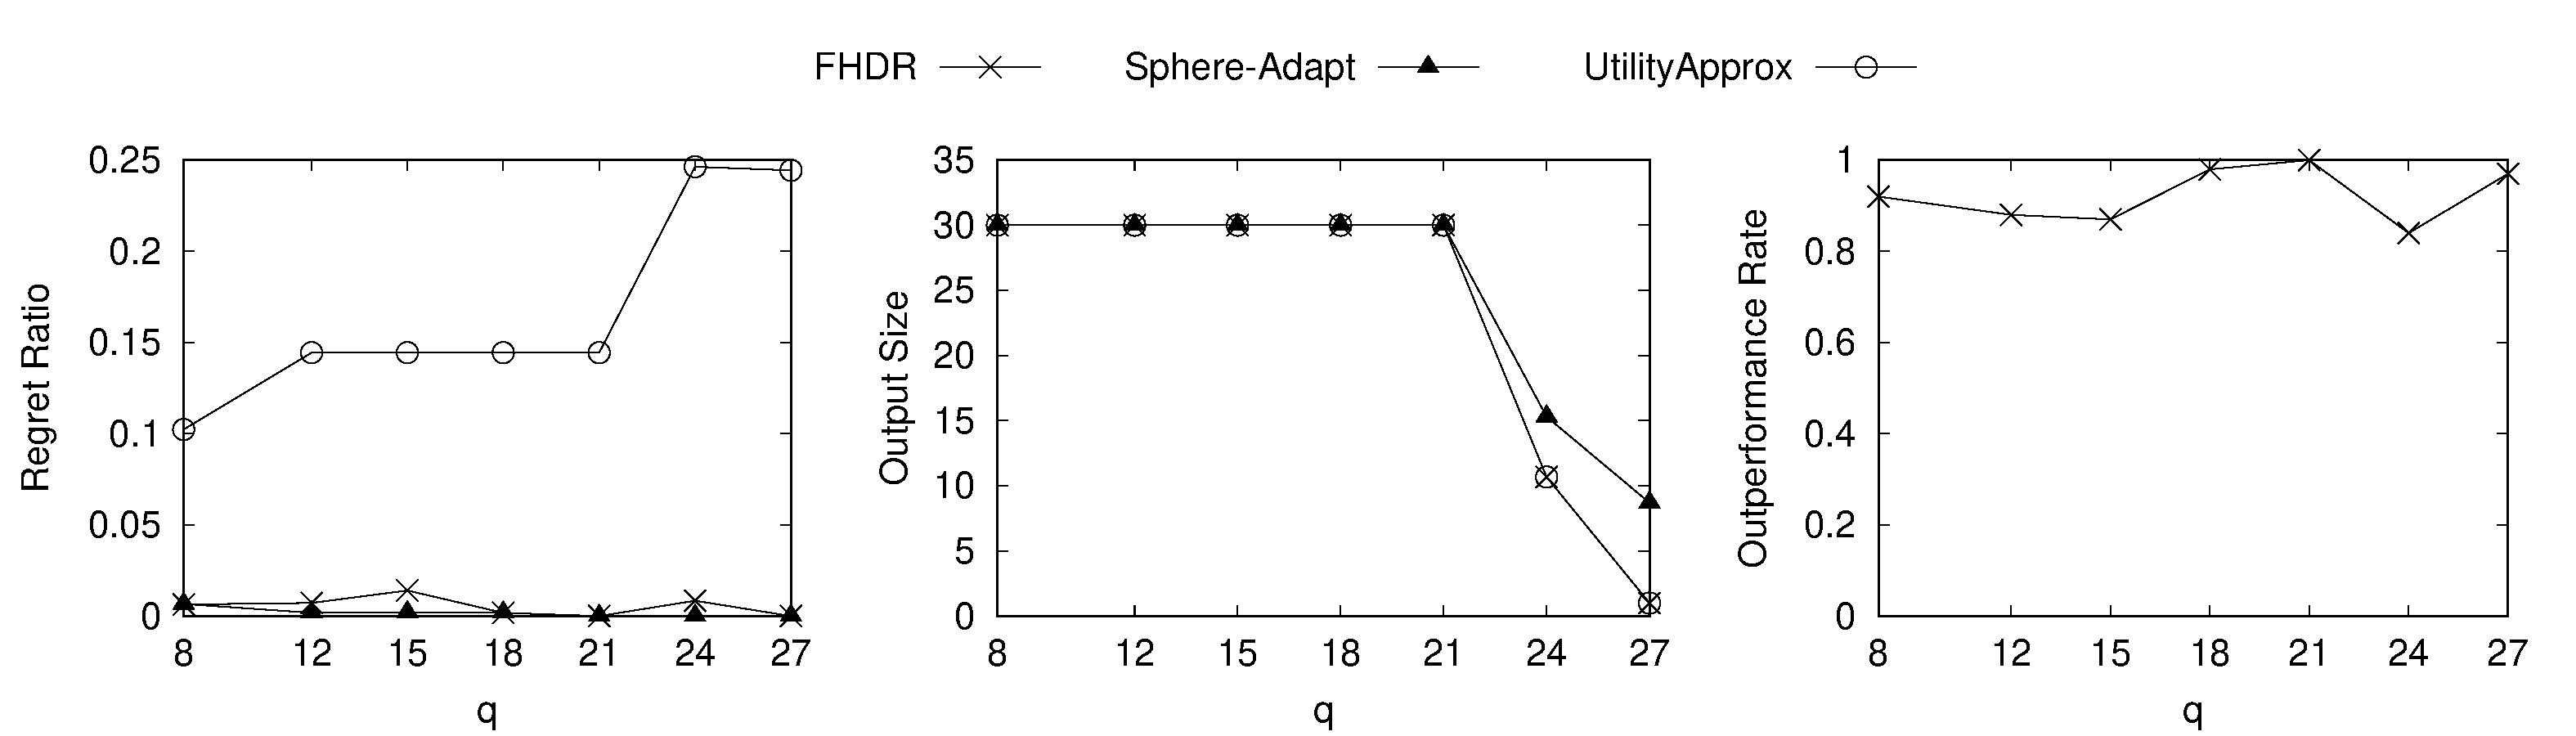
\includegraphics[width=\linewidth]{plot/real/activity/q_plots.pdf}
    \caption{P2: Vary $q$}
    \label{fig:activity_d}
  \end{subfigure}

  \caption{Results on \textit{Activity} dataset}
  \label{fig:activity}
\end{figure*}

\section{Supplementary Material for Experimental Setting}
\label{appen:setting}

\usetikzlibrary{positioning}

\begin{figure*}[tbp]
  \centering
  \begin{tikzpicture}
    \node[inner sep=0] (img) {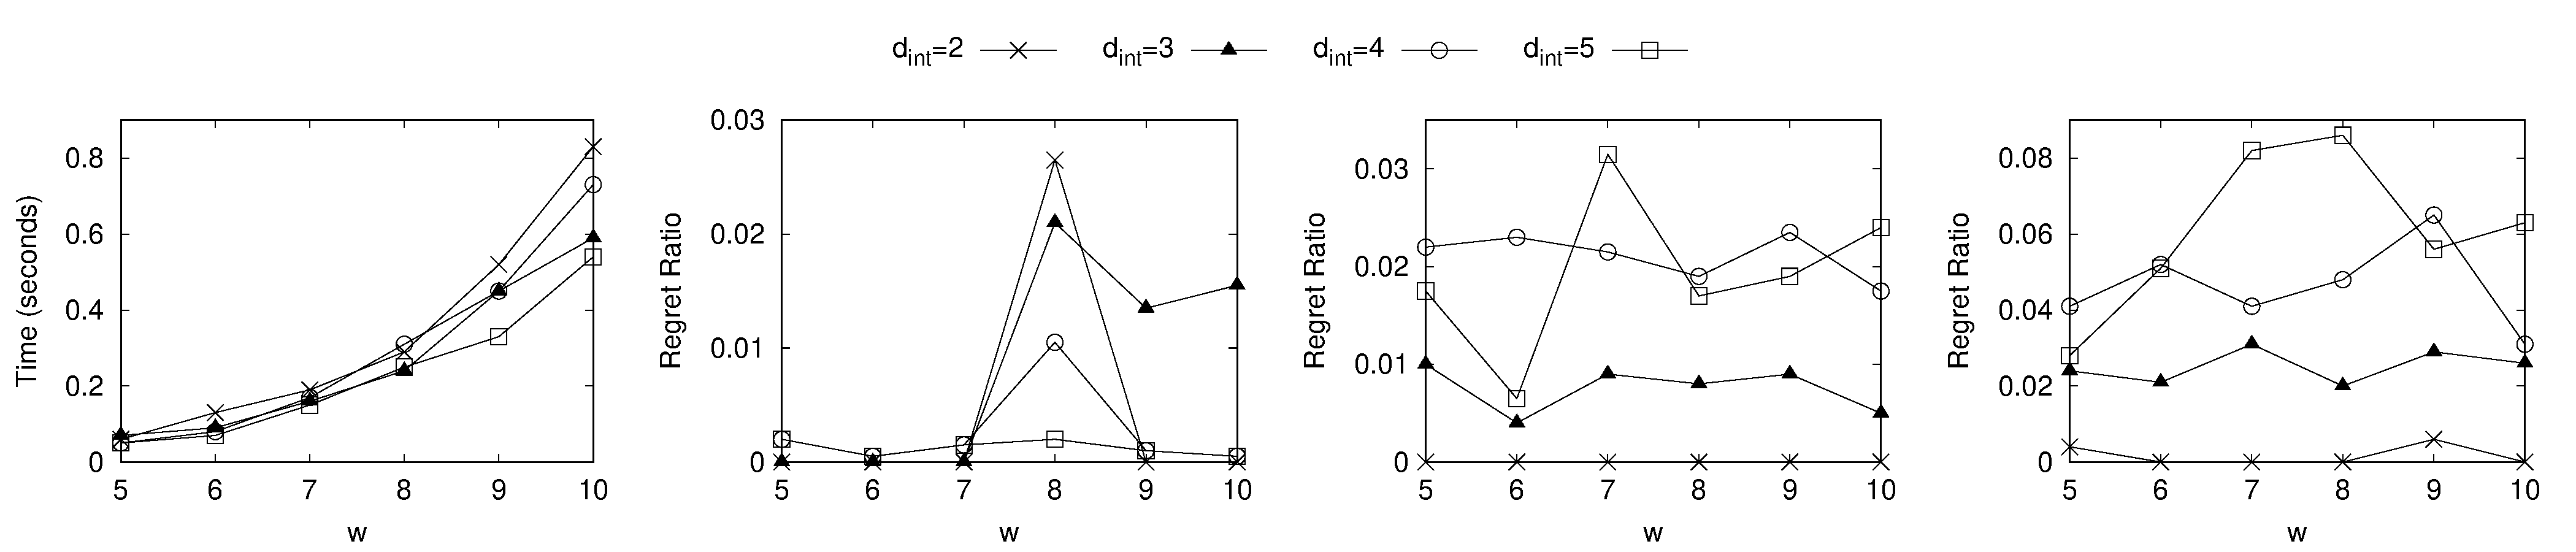
\includegraphics[width=\linewidth]{plot/internal/w.pdf}};

    \path (img.south west) -- (img.south east)
      coordinate[pos=.135] (c1)
      coordinate[pos=.395] (c2)
      coordinate[pos=.643] (c3)
      coordinate[pos=.89] (c4);

    \node[below=2mm of c1, anchor=north, xshift=0pt]  {(Energy)};
    \node[below=2mm of c2, anchor=north, xshift=0pt]  {(Car)};
    \node[below=2mm of c3, anchor=north, xshift=0pt]  {(NBA)};
    \node[below=2mm of c4, anchor=north, xshift=0pt]  {(Energy)};
  \end{tikzpicture}

  \caption{Vary $w$}
  \label{fig:w}
\end{figure*}

\begin{figure}[tbp]
  \centering

  \begin{minipage}[t]{0.54\linewidth}
    \centering
    \renewcommand{\arraystretch}{1.2}
    \vspace{0pt}
    \begin{tabular}{|c|c|c|}
      \hline
      Dataset & $d$ & $|X|$ \\
      \hline\hline
      House  & 33  & 15{,}171 \\
      \hline
      Car    & 57  & 5{,}500 \\
      \hline
      NBA    & 104 & 4{,}790 \\
      \hline
      Energy & 149 & 36{,}043 \\
      \hline
      Activity & 54 & 2{,}872{,}533 \\
      \hline
    \end{tabular}
    \captionof{table}{Real Datasets}
    \label{tab:real-datasets}
  \end{minipage}
  \hfill
  \begin{minipage}[t]{0.42\linewidth}
    \centering
    \vspace{0pt}
    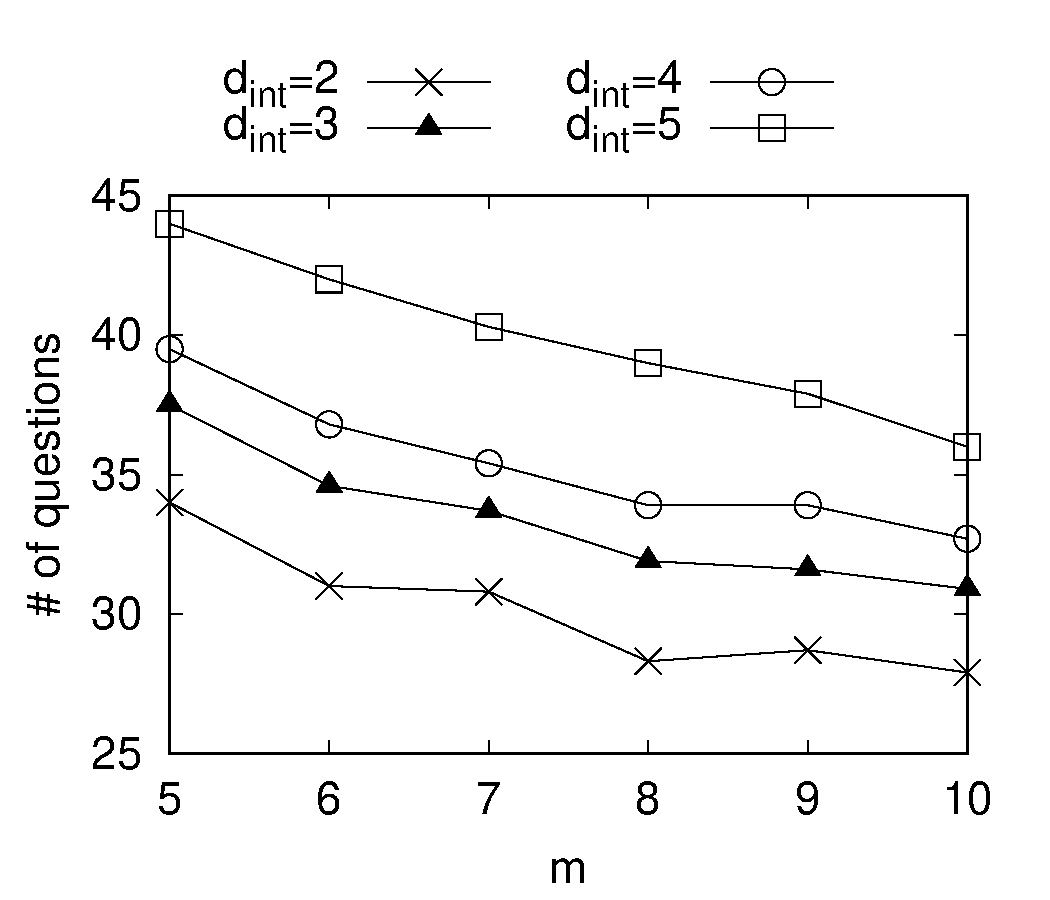
\includegraphics[width=\linewidth]{plot/internal/m.pdf}
    \captionof{figure}{Vary $m$}
    \label{fig:m}
  \end{minipage}

\end{figure}

We evaluate internal parameter choices in terms of regret ratio and execution time.

To assess $m$, we measure the number of questions required to identify the single tuple with the highest utility. As observed in Figure \ref{fig:m}, the number of questions required to identify the optimal tuple decreases as $m$ increases, since each question yields more information. However, a larger $m$ also makes each question more cognitively demanding for the user. We must balance these factors, as both the number of questions and the number of attributes per question contribute to overall cognitive load. Cognitive science literature indicates that humans can only comfortably process a limited number of items at once (e.g., $7$ as suggested by \cite{MG56}), and recent working memory studies find capacity constraints on the order of $4\sim 7$\cite{Morra2024}. In parallel, marketing research guidelines for conjoint analysis recommend using roughly $5\sim7$ attributes at most in each task to avoid overwhelming respondents \cite{McCullough2007}, also supported by some consumer research \cite{OA14, GS78}. Therefore, we use $m$ at 7 in our approach, as this upper limit balances query efficiency in our algorithm with user cognitive limits, aligning with the above guidelines.

For $w$, we restrict the number of questions so that the algorithm can only finish Phase 1, to evaluate performance in \textsc{AttributeSubset}. We plot the execution time on the Energy dataset, and the regret ratio on three datasets (from left to right): Car, NBA, Energy. Results are presented in Figure \ref{fig:w}. As shown in the first plot, the execution time increases sharply once $w$ exceeds $6$. Regarding the regret ratio, a larger $w$ raises the likelihood of including the \textit{key} attributes within each sampled subset, while simultaneously reducing the accuracy upon successfully including all \textit{key} attributes. These two effects counterbalance each other, leading to a more intricate, non-monotonic curve rather than a steady trajectory. In particular, there is a local valley at $w=6$, followed by a peak around $w=7\sim 8$. Based on the overall performance, we select $w=6$ that achieves both efficiency and accuracy.

\section{Additional Statistics of User Study}
\label{appen:user_study}

\begin{table}[t]
\small
\centering
\caption{User study results}
\label{tab:statistics_user_study}
\resizebox{\columnwidth}{!}{
\begin{tabular}{c|ccc|ccc|cc|c}
\toprule
\textbf{P}
& \multicolumn{3}{c|}{\textbf{FHDR}}
& \multicolumn{3}{c|}{\textbf{UH-Random}}
& \multicolumn{2}{c|}{\textbf{Mech. Rate}}
& \textbf{Pref.} \\
\cmidrule(lr){2-4}
\cmidrule(lr){5-7}
\cmidrule(lr){8-9}
& A & S & T & D & A & T & F & S & \\
\midrule

1  & 30 & 20 & 147 & 3 & 4  & 57  & 6  & 4  & F \\
2  & 13 & 8  & 119 & 6 & 10 & 86  & 10 & 10 & U \\
3  & 0  & 0  & 0   & 2 & 4  & 59  & 4  & 7  & B \\
4  & 0  & 0  & 0   & 3 & 7  & 92  & 5  & 7  & B \\
5  & 2  & 1  & 15  & 3 & 4  & 72  & 6  & 6  & U \\
6  & 3  & 1  & 18  & 3 & 3  & 49  & 8  & 8  & F \\
7  & 16 & 9  & 74  & 4 & 8  & 124 & 9  & 7  & F \\
8  & 0  & 0  & 0   & 2 & 5  & 57  & 6  & 5  & U \\
9  & 30 & 12 & 198 & 4 & 7  & 98  & 7  & 7  & F \\
10 & 27 & 15 & 108 & 3 & 8  & 99  & 6  & 5  & B \\
11 & 13 & 6  & 98 & 4 & 8  & 102 & 7  & 6  & F \\
12 & 12 & 6  & 67  & 6 & 6  & 67  & 7  & 6  & F \\
13 & 0  & 0  & 0   & 3 & 6  & 91  & 7  & 3  & U \\
14 & 30 & 11 & 189 & 5 & 8  & 132 & 8  & 9  & U \\
15 & 9  & 6  & 90  & 3 & 6  & 64  & 8  & 8  & F \\
16 & 13 & 9  & 82  & 7 & 7  & 88  & 6  & 3  & F \\
17 & 9  & 6  & 52  & 2 & 5  & 77  & 7  & 6  & F \\
18 & 15 & 5  & 112 & 3 & 7  & 85  & 5  & 6  & B \\
19 & 10 & 5  & 45  & 4 & 6  & 99  & 5  & 8  & U \\
20 & 5  & 3  & 21  & 5 & 11 & 76  & 7  & 7  & F \\
21 & 33 & 21 & 182 & 3 & 8  & 117 & 9  & 4  & F \\
22 & 1  & 1  & 9   & 5 & 7  & 73  & 9  & 5  & F \\
23 & 31 & 21 & 110 & 3 & 9  & 112 & 10 & 5  & F \\
24 & 28 & 7  & 217 & 5 & 9  & 112 & 9  & 9  & F \\
25 & 32 & 15 & 174 & 2 & 7  & 77  & 4  & 8  & U \\
26 & 5  & 3  & 76  & 5 & 12 & 114 & 8  & 7  & F \\
27 & 28 & 9  & 176 & 3 & 9  & 119 & 7  & 5  & F \\
28 & 31 & 8  & 199 & 7 & 12 & 150 & 8  & 6  & F \\
29 & 0  & 0  & 0   & 4 & 7  & 86  & 8  & 8  & U \\
30 & 12 & 6  & 81  & 4 & 8  & 81  & 7  & 6  & F \\

\midrule
\textbf{AVG}
& 14.60
& 7.13
& 88.63
& 3.87
& 7.27
& 90.50
& 7.10
& 6.37
& $\substack{\mathrm{F}:18\\\mathrm{U}:8\\\mathrm{B}:4}$ \\

\bottomrule
\end{tabular}
}
\end{table}

We gathered $30$ participants for the user study, mostly university students. Detailed statistics from the user study are presented in Table \ref{tab:statistics_user_study}. The two main parts in the table, \textsc{FHDR} and \textsc{UH-Random}, records detailed statistics of a specific user using the algorithm. Due to limited space, we denote `P' as participant, `A' as the number of questions answered (including those being skipped), `S' as the number of skipped questions, `T' as the recorded time using the algorithm in seconds, including upfront attribute selection for \textsc{UH-Random}, and 'D' as the number of attributes selected for the \textsc{UH-Random} algorithm, as required. For FHDR sessions with no questions, $T=0$ denotes zero interaction time. Both algorithms contain only three columns: \textsc{FHDR} contains (A,S,T) as we do not know the number of attributes that the user considers implicitly while using the algorithm, and \textsc{UH-Random} contains (D,A,T) since skipping is not allowed. The remaining columns report the ratings of the two interaction mechanisms and the preference over recommendations returned by \textsc{FHDR} and \textsc{UH-Random}.

Upfront attribute-selection time for \textsc{UH-Random} was explicitly measured at approximately $50$~s and is included in its mean total time of $90.50$~s. FHDR’s mean recorded time is $88.63$~s. While the total times are similar, FHDR avoids upfront attribute selection and allows users to skip questions or stop answering at any time. Participants $3$, $4$, $8$, $13$, and $29$ requested recommendations without answering questions and received \textsc{AttributeSubset} outputs. Their $T=0$ entries denote zero interaction time. Other participants skipped questions during interaction, illustrating the use of FHDR’s flexible feedback options. Finally focusing on the preference over the final results, most participants favor the recommendation of our algorithm, which is either more accurately reflecting their preference, or could cover some preferred options successfully.

